\documentclass[11pt,a4paper,twoside]{tesis}
% SI NO PENSAS IMPRIMIRLO EN FORMATO LIBRO PODES USAR
%\documentclass[11pt,a4paper]{tesis}

\usepackage[toc,page]{appendix}

\usepackage{color}
\usepackage{array}


\usepackage{longtable}
\usepackage{graphicx}
\usepackage{float} % para settear posicion a imagenes
\usepackage[utf8]{inputenc}
\usepackage[spanish]{babel}
\usepackage[left=3cm,right=3cm,bottom=3.5cm,top=3.5cm]{geometry}
\usepackage{hyperref} %Para poner link en toc. Creo que tambien para los hrefs en azul
\hypersetup{colorlinks,    citecolor=black,    filecolor=black,    linkcolor=red,    urlcolor=black}
\usepackage{multirow}
\usepackage{bookmark}
%\usepackage{titlesec} 
%\usepackage{sectsty}

%header configuration
\usepackage{titlesec}%Para configurar el formato de los headers (section, subsection, etc)

\titleformat*{\section}{\LARGE\bfseries}
\titleformat*{\subsection}{\Large\bfseries}
\titleformat*{\subsubsection}{\large\bfseries}
\titleformat*{\paragraph}{\large\bfseries}
\titleformat*{\subparagraph}{\large\bfseries}
%end header configuration

%\subsubsectionfont{\large}

\setcounter{tocdepth}{4} % Si se muestra subsubsection o no en el toc
\setcounter{secnumdepth}{4}

\newcommand\dblquote[1]{\textquotedblleft #1\textquotedblright}
\newcommand\sglquote[1]{\textquoteleft #1\textquoteright}
\newcommand\dq[1]{\textquotedblleft #1\textquotedblright}
\newcommand\sq[1]{\textquoteleft #1\textquoteright}

\newcommand*{\allref}[1]{\ref{#1} \nameref{#1}}

\renewcommand{\appendixname}{Apéndices}
\renewcommand{\appendixtocname}{Apéndices}
\renewcommand{\appendixpagename}{Apéndices}
%\usepackage[nottoc,numbib]{tocbibind}

\begin{document}

%%%% CARATULA
\def\autor{Julián Peller}
\def\titulo{Prototipo de Question Answering bilingüe closed y open domain}
\def\runtitulo{Prototipo de Question Answering bilingüe para closed y open domain}
\def\runtitle{Prototipo de Question Answering bilingüe para closed y open domain}
\def\director{José Castaño}
%\def\codirector{Master Yoda}
\def\lugar{Buenos Aires, 2013}
\input{caratula}

%%%% ABSTRACTS, AGRADECIMIENTOS Y DEDICATORIA
\frontmatter
\pagestyle{empty}
%\begin{center}
%\large \bf \runtitulo
%\end{center}
%\vspace{1cm}
\chapter*{\runtitulo}
Question answering es un área de ciencias de la computación que busca generar respuestas concretas a preguntas expresadas en algún lenguaje natural. Es un área compleja que combina herramientas de búsqueda y recuperación de la información (\textit{information retrieval}), de procesamiento del lenguaje natural (\textit{nlp}) y de extracción de información (\textit{information extraction}). Por poner un ejemplo: para el input \textit{\dq{?`Cuándo nació Noam Chomsky?}} un sistema de question answering debería devolver algo como \dq{\textit{el 7 de diciembre de 1928}}.
Este área representa el paso lógico posterior a los sistemas de recuperación de documentos y logró en los último años una serie de hitos impulsados por el proyecto general de la web semántica. Watson, el sistema desarrollado por IBM que derrotó a los mejores competidores de Jeropardy! es el ejemplo más visible, pero incluso buscadores como Bing! y Google comienzan a incorporar este tipo de algoritmia.

En esta tesis investigamos los distintos problemas que se subsumen bajo el concepto de question answering y reseñamos diferentes soluciones y modelos aplicados para resolverlos, bajo el proyecto de la implementación de dos sistemas básicos de question answering. El primer sistema implementado es un modelo de dominio cerrado (específico) y datos estructurados solo para inglés. El segundo modelo es un sistema multilingüe, de dominio abierto y que utiliza como corpora las wikipedias de diferentes idiomas. Para el primer modelo orientamos nuestro desarrollo de acuerdo al modelo teórico del paper \cite{QADB1} e implementamos soluciones para un conjunto restringido de preguntas.  Para el segundo modelo utilizamos  un subconjunto de los problemas de la competencia CLEF '07 y desarrollamos el sistema utilizando como baseline el framework Qanus, adaptándolo para utilizar herramientas de procesamiento de lenguaje multilingües de la librería Freeling.
\bigskip

\noindent\textbf{Palabras claves:} Question Answering, Closed Domain, Open Domain, Multilenguaje, Information Retrieval, Question processing, Procesamiento del lenguaje natural, Freeling, Qanus, CLEF

\cleardoublepage
%%\begin{center}
%\large \bf \runtitle
%\end{center}
%\vspace{1cm}
\chapter*{\runtitle}
Question answering is a computer science area that aims to generate concrete responses to questions posed in some natural language. It's a complex area that combines information retrieval, natural language processing and information extraction tools. For example, for the input \textit{\dq{`When was Noam Chomsky born?}}, a question answer system should return something like \dq{\textit{December 7th, 1928}}.
This area represents a logical step beyond the standard information retrieval systems and in the recent years it has achieved a serie of important milestones, driven by the general project of semantic web. Watson, the system developed by IBM which defeated the best human competitors of Jeopardy! is the most visible example, but even search engines like Bing! and Google have started to incorporate this kind of algorithmics.

In this thesis we research the different problems subsumed under the concept of question answering and we reviews different solutions and models applied to resolve them, under the project of the implementation of two basic systems of question answering. The first implemented system is a closed (specific) domain model with structured data only for English. The second model is a open domain multilingual system which uses as corpora wikipedias in different languages. For the first model we oriented our develpmnet following the theoretical framework exposed in the paper \cite{QADB1} and we implemented solutions for a restricted set of questions. For the second model, we used a subset of problems of the competition CLEF '07 and we developed the system using as baseline the framework Qanus, adapting it to use the multilingual natural language processing tools of the library Freeling.
\bigskip

\noindent\textbf{Keywords:} Question Answering, Closed Domain, Open Domain, Multilingual, Freeling, Qanus, CLEF, Semantic Tractability

%\cleardoublepage
%\chapter*{Agradecimientos}

\noindent A mi Chiche Hellbun.
 % OPCIONAL: comentar si no se quiere

%\cleardoublepage
%\hfill \textit{A mi madre y al Estado Nacional, por estar cuando hizo falta.}  % OPCIONAL: comentar si no se quiere

%\cleardoublepage
\tableofcontents

\mainmatter
\pagestyle{headings}

%%%% ACA VA EL CONTENIDO DE LA TESIS


\chapter{Introducción}
\label{chap:intro}\label{chap:1}


\section{Qué es question answering}
\label{sec:que-es-qa}
% Estado: Cerrado. Contenido y formato está OK, ortografía está corregida.

Question answering es un área de ciencias de la computación que busca generar respuestas concretas a preguntas expresadas en algún lenguaje natural. Es un área compleja que combina herramientas de búsqueda y recuperación de la información (\textit{information retrieval}), de procesamiento del lenguaje natural (\textit{PLN}) y de extracción de información (\textit{information extraction}). Por poner un ejemplo: para el input \textit{\dq{?`Cuándo nació Noam Chomsky?}} un sistema de question answering podría devolver \dq{\textit{7 de diciembre de 1928}}.
Este área representa el paso lógico posterior a los sistemas de recuperación de documentos y logró en los último años una serie de hitos impulsados por el proyecto general de la web semántica. Watson, el sistema desarrollado por IBM que derrotó a los mejores competidos de Jeropardy! en tiempo real\footnote{En esta url está disponible el programa en el que el sistema vence a sus competidores humanos: \url{http://www.youtube.com/watch?v=WFR3lOm_xhE}} es el ejemplo más visible, pero incluso buscadores como Bing! y Google comienzan a incorporar este tipo de algoritmia.

Los sistemas de question answering suelen ser sistemas complejos que abordan distintas problemáticas: por un lado deben definir y optimizar la base de conocimiento para el dominio dado, por otro deben realizar un análisis de las preguntas en lenguaje natural a fin de volverlas
tratables computacionalmente y, finalmente, deben poder buscar -o generar- y decidir la mejor respuesta para la pregunta ingresada, si es que esa respuesta existe.

Algunos de estos subproblemas tienen nombre propio en la literatura y son un sub-área específica. Por ejemplo, dependiendo de la amplitud de la base de conocimiento, un sistema es de dominio cerrado (\textit{closed domain}), si la base es acotada a un dominio de la realidad específico; por el contrario se llama de dominio abierto (\textit{open domain}), si no lo es, es decir, si se espera que sepa responder preguntas de cualquier dominio. Por su parte, dominios de conocimiento más pequeños, en general, requieren y permiten un modelado más exhaustivo
de los datos y un análisis más estructurado, mientras que dominios de conocimiento más abiertos suelen
tener un enfoque apoyado más fuertemente en el análisis lingüístico cuantitativo.

Otra distinción usual contempla el tipo de datos de la base de conocimiento:  puede ser estructurado, como en una base de datos
relacional, semi-estructurado, como los documentos XML, o también sin estructura, como el texto plano. Cada tipo de datos tiene su enfoque:
los datos estructurados definen una ontología acotada que limita qué cosas se pueden preguntar y, en consecuencia, qué cosas se pueden responder: el problema en este caso consiste en traducir la pregunta formulada en un lenguaje humano a una consulta válida definida en el modelo de datos. Por otro lado, si los datos no tienen estructura, no es posible definir una ontología rígida y se hace necesario otro tipo de enfoque más difuso y basado en análisis lingüísticos del corpus de datos mismo contra la pregunta. No siempre,  pero en general una base de conocimiento closed domain está asociada a un tipo de datos estructurado o semi-estructurado, mientras que las bases open domain suelen ser no estructuradas.

Otro tipo de clasificación se centra en el tipo de preguntas que los sistemas saben responder. Los tipos más conocidos son las factoids -o fácticas-, que refieren a hechos fácticos (¿Cuándo ocurrió ...? ¿Cuántos hijos tiene...? ¿En dónde vivía Y en el año ...?), las listas (¿Qué libros escribió Nietzsche entre 1890 y 1900?) y las definiciones (¿Qué es un huracán?). Otros tipos usuales son las preguntas por un modo (¿Cómo...?), por una razón (¿Por qué...?) y, en general, pueden agregarse subclasificaciones como dependencias temporales explícitas o dependencias semánticas con otras preguntas.

En \allref{chap:estado-de-arte} veremos con detalle los enfoques arquitecturales usuales del área y los componentes típicos de cada módulo.

\section{Proyecto de la tesis}
\label{sec:proyecto}
% Estado: Cerrado. Contenido y formato está OK, ortografía está corregida.

En esta tesis investigamos los distintos problemas que se subsumen bajo el concepto general de question answering y reseñamos diferentes soluciones y modelos aplicados para resolverlos, todo esto bajo el proyecto general de la implementación de dos modelos de question answering: uno de dominio cerrado, específico, y datos estructurados en inglés, por un lado, y otro sistema multilingüe, de dominio abierto y que utiliza como corpus las wikipedias de diferentes idiomas, por el otro. Para el primer modelo orientamos nuestro desarrollo de acuerdo al modelo teórico del paper \cite{QADB1} e implementamos soluciones para un conjunto restingido de preguntas. Para el segundo modelo utilizamos   un subconjunto de los problemas de la competencia CLEF '07 y desarrollamos el sistema utilizando como baseline el framework Qanus, adaptándolo para utilizar herramientas de procesamiento de lenguajes multilingües de la librería Freeling.

Mientras el enfoque estructurado es complicado de evaluar debido a su dominio acotado y específico, es más sencillo realizar experimentos sobre las herramientas al utilizarlas en el modelo no estructurado, gracias a las distintas competencias cuya razón de ser es, justamente, la creación de criterios de evaluación al nivel de la comunidad de investigadores del área. Los resultados tangibles de esta tesis son dos modelos de software con diferentes soportes para idiomas: un modelo básico de question answering como interfaz a la base de datos en inglés, montado sobre una base de datos con información de países y ciudades de ejemplo, y un modelo no estructurado de dominio abierto, completamente multilingüe, que resuelve algunas subtareas de la competencia Clef '07.


Con un poco más de detalle, la implementación del modelo de dominio cerrado está basada en los trabajos de Ana María Popescu et. al.  \cite{QADB1} y \\
\cite{QADB2} en donde se define la noción de pregunta \textit{semánticamente tratable} en el contexto de una base de datos concreta. Proponen allí, así mismo, un modelo teórico para identificar este tipo de preguntas y una forma de transformarlas en consultas de SQL, así como también un sistema concreto que implementa el modelo. Popescu argumenta que una interfaz a una base de datos en lenguaje natural puede no identificar una pregunta, pero que jamás debe mal interpretarla activamente, es decir, interpretar algo distinto a lo preguntado y dar una respuesta que no se condice con la necesidad de información del usuario. Una mala interpretación de una pregunta reducirá la confianza del usuario en el sistema, volviéndolo inusable. En cambio, identificando una pregunta como intratable, se puede disparar un proceso de reformulación o especificación asistida de la pregunta, lo cual no es tan costoso en términos de confianza en el sistema. La idea principal que guía a sus trabajos es proponer una clase de preguntas específica que sea 1) suficientemente sencilla para ser interpretada por un modelo computacional y, a la vez, suficientemente abarcadora de las preguntas generalmente hechas por humanos. La intuición detrás de este enfoque es que, mientras, en el caso general, una pregunta puede ser compleja, ambigüa y difícil de comprender (incluso por un humano), también hay preguntas simples, unívocas y con una interpretación sencilla incluso para una máquina (por ejemplo: ``¿Qué restaurantes de comida china hay en Belgrano?''). La \textit{tratabilidad semántica}, cualidad de una pregunta para una base de datos dada, define esta clase de preguntas simples. Nosotros implementamos una versión limitada de este modelo teórico en \allref{chap:4} sobre un la base de datos World\footnote{Ver \url{http://dev.mysql.com/doc/world-setup/en/index.html} y \url{http://dev.mysql.com/doc/index-other.html}} (ver \allref{sec:popescu-db}), provista por mysql, que consiste en tres tablas (countries, cities y languages), y posee cierta información básica de geografía internacional.

Por su parte, para desarrollar y evaluar mecanismos de dominio abierto resolvimos algunos ejercicios de la competencia de question answering organizada por CLEF
en 2007. CLEF (de \textit{Cross-Language Evaluation Forum}) es una organización que busca fomentar la investigación en sistemas de information retrieval cross-language. En particular, una vez por año CLEF lanza una competencia de Question Answering multilingüe, con diferentes corpus y diferentes tipos de ejercicios. Estas competencia permiten obtener un patrón estándar de comparación entre distintos desarrollos y una idea general del estado de arte alcanzado en cada área.
Por ejemplo, la competencia ya finalizada del año 2013, QA4MRE@CLEF2013, (Question Answering for Machine Reading Evaluation) se enfoca principalmente en Machine Reading, tarea que incluye un grado de razonamiento elevado para la computadora\footnote{\url{http://celct.fbk.eu/QA4MRE/}}. Existen distintas conferencias de evaluación de sistemas QA o de subtareas asociadas (por ejemplo TREC - Text Retrieval Conference \footnote{\url{http://trec.nist.gov/}}-, TAC - Text Analysis Conference \footnote{\url{http://www.nist.gov/tac/}}) - y, a su vez, estas distintas competencias ofrecen distintos llamados a competencias. Elegimos resolver una tarea de la competencia Clef '07  por varias razones (Ver \cite{GuidelineClef07} y \cite{OverviewClef07} para un detalle exhaustivo de la conferencia en cuestión). La razón principal fue la pertinencia de la tarea a evaluar al scope de esta tesis. Muchas competencias exigen un grado de complejidad que excede por mucho lo que puede alcanzarse en el tiempo estimado de una tesis de licenciatura y, si bien tuvimos que recortar ciertos aspectos de las tareas a fin de implementar este proyecto en tiempo y forma, estos aspectos fueron pocos.
Otra razón fue la disponibilidad y el atractivo de la base de conocimiento para estos ejercicios: utilizan imágenes de wikipedia.
La competencia del '07 ofrece dos tipos de tareas:
\begin{itemize}
\item Monolingual: donde el idioma de la pregunta y el idioma de la fuente de información son el mismo.
\item Cross-lingual: donde el idioma de la pregunta y el idioma de la fuente de información difieren.
\end{itemize}
Las tareas consideran los siguientes idiomas: inglés, búlgaro, alemán, español, italiano, francés, holandés, rumano y portugués. Por su parte, algunos problemas utilizan corpus de datos privados de la competencia y otros utilizan como fuente las distintas wikipedias. De los problemas que utilizan wikipedia, implementamos un sistema que responde las preguntas en español, mono-idioma, es decir, ejercicios con preguntas formuladas en español que se responden en base a la wikipedia en español e hicimos lo mismo para el portugués.
A su vez, implementamos esta misma solución para el inglés, dado que estaban disponibles las preguntas y señalados los links a las imágenes de wikipedia en inglés, pero no fue posible evaluar sus resultados debido a que las respuestas esperadas no estaban disponibles online y no obtuvimos respuesta de los organizadores de la competencia. El uso estructural de la librería freeling permite la implementación de soluciones para otros idiomas mediante el set-up del corpus en el idioma y una pequeña configuración.
Los ejercicios elegidos constan de 200 preguntas agrupadas. Los grupos de preguntas refieren a un tema, inferible a partir de la primer pregunta.
Por ejemplo, el primer grupo de preguntas es:
\begin{itemize}
\item ¿En qué colegio estudia Harry Potter?
\item ¿Cuál es el lema del colegio?
\item ¿En qué casas está dividido?
\item ¿Quién es el director del colegio?
\end{itemize}
Es decir, para cada grupo se debe inferir el \dq{tema} en la primer pregunta para arrastrarlo a la hora de responder las siguientes. Más allá de esta particularidad, las preguntas son preguntas simples. Más adelante haremos un análisis de las mismas con más detalle.



\section{Estructura de la tesis}
\label{sec:estructura}
% Estado: Falta cerrar definitivo cuando esté completa la tesis, ya que versa sobre su estructura concreta.
% Estado: De lo existente, el contenido y formato está OK, ortografía está corregida.

La tesis se articula de la siguiente manera: En la Introducción (\ref{chap:1}), que estamos concluyendo en estos párrafos, realizamos en primer lugar una introducción mínima al área del question answering (\ref{sec:que-es-qa}), en segundo lugar mencionamos los alcances de esta tesis (\ref{sec:proyecto}), y en tercer lugar, aquí, damos una estructura general de la tesis (\ref{sec:estructura}).

En el siguiente capítulo (\ref{chap:teorico}) recorreremos los conceptos generales de algunas áreas en las que se apoya question answering, repasando primero la terminología básica (\ref{sec:terminologia}) para pasar luego a comentar estructuras típicas de recuperación de la información (\ref{sec:information-retrieval}) y, finalmente, de procesamiento de lenguajes (\ref{sec:nlp}) aplicado a problemas de question aswering.

En el capítulo III (\ref{chap:estado-de-arte}) pasamos revista general del estado de arte del área. Primero realizamos una introducción general (\ref{sec:intro-general-qa}), considerando la historia de la disciplina, las competencias en las que la investigación se nucleó (\ref{subsec:historia}) y las métricas utilizadas por estas competencias para evaluar a los competidores (\ref{subsec:metricas}), luego hacemos un recorrido de diferentes enfoques, considerando el estado de arte académico para dominio abierto (\ref{subsec:open-domain}) y dominio cerrado (\ref{subsec:closed-domain}) y finalmente, el comercial, reseñando el funcionamiento de Watson de IBM (\ref{subsec:ibm-watson}).

En los siguientes capítulos presentamos los modelos implementados:

En el IV (\ref{chap:4}) comentamos el modelo de dominio cerrado para la base de datos World, presentando primero la base de datos (\ref{sec:popescu-db}) y luego la implementación de nuestro sistema (\ref{sec:popescu-implementacion}), pasando revista de su código (\ref{subsec:popescu-codigo}), dando ejemplos (\ref{subsec:popescu-ejemplos}) y presentando conclusiones, limitaciones y trabajo futuro(\ref{subsec:popescu-cierre}).

En el V (\ref{chap:5}) presentamos el modelo de dominio abierto para las wikipedias de diferentes idiomas, presentando en primer lugar los problemas seleccionados de la competencia Clef '07 (\ref{sec:ejercicio-de-clef}), en segundo lugar la implementación de nuestro sistema (\ref{sec:sistema}), presentando el sistema baseline de basado en Qanus (\ref{subsec:baseline}), las adaptaciones multilingües y demás mejoras realizadas (\ref{subsec:modificaciones}), las diferentes corridas que realizamos para evaluarlo (\ref{sec:eval}) y, finalmente, las conclusiones, los límites y potenciales mejoras del sistema (\ref{sec:clef-cierre}).
\chapter{Marco teórico}
\label{chap:teorico}
\section{Términos básicos}

\subsection*{Tokens}

Un token es una palabra o un signo de puntuación en el contexto de un
texto.

Por ejemplo, el texto {\textquotedblleft}El sol
brilla.{\textquotedblright} tiene cuatro tokens:
\{{\textquoteleft}El{\textquoteright}, {\textquoteleft}sol{\textquoteright}, {\textquoteleft}brilla{\textquoteright}, {\textquoteleft}.{\textquoteright} \}. 
Las herramientas que generan una lista de tokens a partir de un texto se llaman
\textit{tokenizers} y suelen permitir distintos tratamiento de ciertas
palabras o signos de puntuación. Las bibliotecas que proveen
tokenizers proveen también herramientas para dividir un texto en
oraciones. Estos dos procesos son el primer paso de todos los
análisis de procesamiento de lenguaje natural siguientes.


\subsection*{N-Gramas}

Un n-grama es una subsecuencia continua de \textit{n} tokens de un string.

Por ejemplo, la oración: {\textquotedblleft}Hoy está nublado{\textquotedblright}, tiene los siguientes n-gramas:
\medskip

\begin{tabular}{lll}
Tres unigramas & : & \{ {\textquotedblleft}Hoy{\textquotedblright}, {\textquotedblleft}está{\textquotedblright}, {\textquotedblleft}nublado{\textquotedblright} \} \\
Dos bigramas & : & \{ {\textquotedblleft}Hoy está{\textquotedblright}, {\textquotedblleft}está nublado{\textquotedblright} \} \\
Un sólo trigrama & : & \{ {\textquotedblleft}Hoy está nublado{\textquotedblright} \}\\
\end{tabular}
\medskip

Los n-gramas son útiles para recorrer un
texto con distintos tama\~nos de ventana en busca de algún patrón
conocido, por ejemplo: buscando entidades nombradas que no fueron reconocidas por otras herramientas.

\subsection*{Ontología}

El término `ontología' es un término originalmente filosófico, que refiere al estudio de lo que hay, de lo que es, o, dicho de otro modo, a la definición y al estudio de los entes que existen en la realidad última y de sus cualidades esenciales y sus relaciones intrinsecas. Aplicado a ciencias informáticas, principalmente dentro áreas como inteligencia artificial y representación del conocimiento, esta noción original se sostiene, acotando la noción de realidad última a uno o varios dominios de problemas. Más concretamente, la noción de ontología en informática refiere a la definición formal y exhaustiva de un conjunto de conceptos que representan entidades, tipos o clases de entidades, propiedades y relaciones entre estas entidades relevantes para el modelado de un dominio de problemas dado. Esta ontología formal define un vocabulario inicial fijo que determina el tipo de problemas que se pueden plantear (y resolver) para el dominio.

\section{Herramientas}

\subsection{Indice invertido}
Un índice invertido es la estructura de datos típica utilizada en problemas de information retrieval. Consiste en un mapeo de términos en documentos que los contienen. Es decir, para un término dado, un índice invertido devuelve una lista de los documentos cargados que lo contienen. Este tipo de estructuras invierte la relación normal en la cual a partir de un documento se accede a la lista de términos que este documento contiene (de allí el nombre \textit{invertido}).
Por ejemplo, para los textos:
\medskip

\begin{tabular}{lll}
T[0] & = & ``qué es esto" \\
T[1] & = & ``esto es un ejemplo" \\
T[2] & = & ``qué gran ejemplo" \\
\end{tabular}
\medskip

Un índice invertido contendría las siguientes entradas (dónde el número \textit{n} es un puntero al texto T[n]):
\medskip %this skips a bit of vertical space

\begin{tabular}{lll}
	``qué" & : & \{0, 2\}\\
	``es" &:& \{0, 1\}\\
	``esto" & :& \{0, 1\} \\
	``un" & :&   \{1\} \\
	``ejemplo" & :& \{1, 2\} \\
	``gran" & :& \{2\} \\
\end{tabular}
\medskip



\subsection{Part-of-speech (POS) tagging}
\label{subsec:pos}
El POS-tagging o \textit{etiquetado gramatical} consiste en asignar a los diferentes 
tokens una etiqueta con el rol o categoría gramatical que cumplen en su contexto de emisión (por lo general, una oración o un párrafo). 
El POS-tagging cumple un rol fundamental en áreas como el reconocimiento de voz, el procesamiento de lenguaje natural e information retrieval.
El input de un pos tagger es una lista de tokens y un tagset (conjunto de etiquetas) específico, mientras que su output es un tag para cada uno 
de los tokens. Como ejemplo introductorio, consideremos la siguiente oración y un etiquetado gramatical posible:
Para la oración:
\begin{center}
{\textquotedblleft}El hombre bajó la escalera.{\textquotedblright} 
\end{center}
\medskip

El resultado de un POS-tagger podría ser el siguiente:%\newline

\begin{center}
\begin{tabular}{| l | l |}
 \hline
Token & Etiqueta Gramatical (POS-tag) \\ \hline
El  & Determinante, artículo definido, masculino, singular\\ \hline
hombre &  Nombre común masculino singular (sustantivo) \\ \hline
bajó  & Verbo principal indicativo pasado tercera persona del singular (genero indefinido)\\ \hline
la  & Determinante, artículo femenino singular \\ \hline
escalera & Nombre común femenino singular (sustantivo) \\ \hline
.  & Punto final\\ \hline
\end{tabular}
\end{center}

La asignación de etiquetas no es un proceso trivial debido a la ambigüedad de roles posibles que tienen muchas palabras. Por ejemplo, la palabra
\sq{ayuda} puede funcionar como sustantivo (en \dq{La ayuda llegó a tiempo}) o como verbo (en \dq{Batman ayuda a los ciudadanos de Ciudad Gótica}). 
Un algoritmo de pos-tagging debe resolver estas ambigüedades seleccionando la categoría adecuada según el contexto. Más allá de estos casos, muchas palabras tienen una sola categoría posible (por ejemplo: \sq{ventana} es siempre un sustantivo, mientras que \sq{lentamente} es un adverbio y \sq{corrió} un verbo, etc).

Existen diferentes formas de clasificar gramaticalmente a las palabras. El esquema más general y reconocido de categorias gramaticales tal vez sea el siguiente, de 9 clases:
\begin{center}
\begin{tabular}{| l | l |}
 \hline
Categoría General & Ejemplos \\ \hline 
Determinante & aquel, este, mi, sus, nuestras \\ \hline
Pronombre & yo, tú, él, mí, nos, aquéllos, suyos \\ \hline
Preposición & a, ante, bajo, con, contra\\ \hline
Conjunción & y, aunque, pero, incluso\\ \hline
Interjección & ah, eh, ejem\\ \hline
Sustantivo & chicos, tesis, Pedro, cortapapeles\\ \hline
Verbo & cantamos, corrió, bailarán\\ \hline
Adjetivo & alegre, bonita, pésimos, desnuda\\ \hline
Adverbio & despacio, hábilmente, posteriormente\\ \hline
\end{tabular}
\end{center}

Mientas a algunas de estas categorías se les puede agregar más información, como \textit{género} y \textit{número} a los sustantivos, otras son categorías que no toleran modificaciones. Veremos esto con más detalle al hablar del tagset propuesto por el grupo EAGLES en breve.

Si bien en ciertos idiomas estas categorías no resultan del todo adecuadas o explicativas, dentro del scope de esta tesis podemos dejar de lado este problema.
Estas clases de palabras -en general, para muchos idiomas- pueden dividirse en dos superclases conceptuales de acuerdo a su naturaleza: las clases cerradas y las abiertas. Las primeras constan de una lista acotada y fija de palabras y está, por lo general, cristalizada. Esto es: no se incorporan, a esta altura de la historia del lenguaje, nuevas palabras a las clases gramaticales cerradas. Además, estas clases de palabras cumplen un rol funcionaal en la construcción de la oración y, como una nota más, son palabras cortas. Son clases cerradas, de las 9 recién enunciadas, los determinantes, los pronombres, las preposiciones, las conjunciones y las interjecciones. En contraposición, las clases abiertas son los sustantivos, los verbos, los adjetivos y los adverbios. Las clases abiertas incorporan, con naturalidad y frecuencia, nuevas palabras a su lista: se inventan nuevos objetos y en consecuencia nuevos sustantivos y nuevas acciones (nuevos verbos). Existen esquemas formales de conjugación de miembros a las clases abiertas, teniendo la mayoría sus miembros ciertas regularidades morfológicos que se repiten. 

A partir de las clases de lingüística teórica y algunas otras características de la morfología de las palabras se construyen los \textit{tagsets}. Estos son diferentes conjuntos de etiquetas que se utilizan de hecho en los algoritmos de tagging, siendo los más conocidos el tagset de 87 etiquetas usado en el Corpus Brown y algunos de sus derivados: el tagset de Penn Treebank, de 45 tags; el C5, de 61 tags, usado en el proyecto CLAWS y el C7, más grande, de 146 tags. 
El pos tagger de Stanford (usado en esta tesis) utiliza el tagset de Penn Treebank, cuyas etiquetas y significados se listan en la siguiente tabla:

\begin{figure}[H]
  \centering
    \includegraphics[scale=0.3]{graficos/penn-tagset}
  \caption{Tagset Penn Treebank}
  \label{fig:tagset-penn}
\end{figure}

%\newline

Por su parte, el pos-tagger español de Freeling, por su naturaleza multilingüe, utiliza el tagset propuesto por el grupo EAGLES (\textit{Expert Advisory Group on Language Engineering Standards})\footnote{\url{http://www.ilc.cnr.it/EAGLES96/home.html}}, una organización europea que fomenta la investigación multilingüe, mientras que por una cuestión de compatibilidad, se preservan los tags de Penn Treebank para el inglés. Los tags de EAGLES tienen en consideración diferentes matices para contemplar las variaciones de diferentes idiomas. Sobre un conjunto inicial de 12 categorías -las 9 recién enunciadas más \sq{Signos de puntuación}, \sq{Numerales} y \sq{Fechas y horas} define etiquetas mucho más especificas. En concreto, un tag consta de entre 6 y 7  posiciones, cada una de las cuales expresa una caracteristica de la palabra dependiendo del valor especificado en la posición anterior. Para algunas clases alguno de estos valores no tienen sentido, mientras que para algunas palabras algunos valores no están o no pueden definirse (en el caso de subespecificación de un atributo, esta se nota como un \sq{0}). 
A continuación presentamos la especificación para el conjunto de tags relacionados con sustantivos y un ejemplo de su aplicación.

\begin{center}
\begin{tabular}{| l | l | l | l |}
 \hline
 \multicolumn{4}{|c|}{Nombres} \\ \hline
Pos. & Atributo & Valor & Código \\ \hline
1 & Categoría &  Nombre & N \\ \hline
\multirow{2}{*}{2} & \multirow{2}{*}{Tipo} & Común  & C \\ \cline{3-4}
  & &      Propio & P \\ \hline
\multirow{3}{*}{3} & \multirow{3}{*}{Género} & Masculino & M \\ \cline{3-4}
 & & Femenino &  F \\ \cline{3-4}
 & & Común    & C  \\ \hline
\multirow{3}{*}{4} & \multirow{3}{*}{Número} & Singular & S \\ \cline{3-4}
 & & Plural &  P \\ \cline{3-4}
 & & Invariable & N  \\ \hline
 \multirow{4}{*}{5-6} & \multirow{4}{*}{Clasificación Semántica} & Persona & SP \\ \cline{3-4}
 & & Lugar &  G0 \\ \cline{3-4}
 & & Organización &  O0 \\ \cline{3-4}
 & & Otros & V0  \\ \hline
\multirow{2}{*}{7} & \multirow{2}{*}{Grado} & Aumentativo  & A \\ \cline{3-4}
  & & Disminutivo & D \\ \hline
\end{tabular}
\end{center}


\begin{center}
\begin{tabular}{| l | l | l |}
 \hline
Forma & Lema & Etiqueta \\ \hline 
chico & chico & NCMS000 \\ \hline
chicas & chico & NCFP000 \\ \hline
gatito & gato & NCMS00D \\ \hline
oyente & oyente & NCCS000 \\ \hline
oyentes & oyente & NCCP000 \\ \hline
cortapapeles & cortapapeles &NCMN000 \\ \hline
tesis & tesis & NCFN000 \\ \hline
Barcelona & barcelona & NP000G0 \\ \hline
COI & coi & NP000O0 \\ \hline
Pedro & pedro & NP000P0 \\ \hline
\end{tabular}
\end{center}


Existen varios enfoques algoritmicos al problema del POS tagging: desde los más primitivos basados en reglas escritas a mano pasando a los basados en HMMs (Hidden Markov Models), Maximum Entropy o Transformation Based Learning. Un detalle de estos métodos excede la introducción al problema que supone esta sección de la tesis. El POS tagger de Freeling está basado en el approach de HMMs y el de Stanford en el de Maximum Entropy, ambos modelos de machine learning. En \allref{subsec:freeling-pos} y \allref{sec:stanford-pos} se encuentran algunos comentarios más técnico de los algoritmos de POS tagging que utilizamos en este trabajo y vinculos a bibliografía pertinente y en la sección siguente \allref{subsec:nerc} veremos una descripción más detallada de enfoques algorítmicos al problema que ilustrarán, al menos de modo general, la estructura de la algoritmía basada en machine learning aplicada a procesamiento de lenguajes. 
A continuación listamos ejemplos concretos de análisis de la oración de ejemplo del comienzo de esta sección (\dq{El hombre bajó la escalera.}) para mostrar un funcionamiento real de los algoritmos utilizados en esta tesis. 


\begin{center}
\begin{tabular}{| l | l | l |}
\hline
\multicolumn{3}{|c|}{Freeling (ES)} \\ \hline
Forma &  Etiqueta & Descripción \\ \hline 
El & DA0MS0 & Determinante, Artículo, Másculino, Singular\\ \hline 
hombre & NCMS000 & Nombre, Común, Másculino, Singular  \\ \hline 
bajó & VMIS3S0 & Verbo, Principal, Indicativo, Pasado, Tercera Persona, Singular\\ \hline 
la & DA0FS0 & Determinante, Artículo, Femenino, Singular\\ \hline 
escalera& NCFS000 & Nombre, Común, Femenino, Singular \\ \hline 
.& Fp& Punto final\\ \hline \hline
\multicolumn{3}{|c|}{Freeling (EN)} \\ \hline
Forma & Etiqueta & Descripción \\ \hline 
The &DT & Determiner \\ \hline 
man &NN & Noun, singular or mass \\ \hline 
came  &VBD& Verb, past tense\\ \hline 
down  &RP& Particle \\ \hline 
the &DT& Determiner \\ \hline 
stairs & NNS& Noun, plural \\ \hline 
.& Fp& Sentence final punctuation \\ \hline \hline
\multicolumn{3}{|c|}{Stanford (EN)} \\ \hline
Forma & Etiqueta & Descripción \\ \hline 
The &DT & Determiner \\ \hline 
 man & NN & Noun, singular or mass \\ \hline 
  came &VBD  & Verb, past tense \\ \hline 
 down & RP  &  Particle\\ \hline 
 the & DT  &  Determiner \\ \hline 
 stairs. &NN   & Noun, plural \\ \hline 
 \end{tabular}
\end{center}

En el scope de este proyecto, utilizamos pos-tagging para filtrar clases de palabras inútiles y para seleccionar tres tipos: las qwords, los verbos y los sustantivos (Las qwords son los pronombres interrogativos: qué, quién, cómo, etc. y en inglés, who, when, where...). \newline


\subsection{Named Entity Recognition (NER)}
\label{subsec:nerc}
El reconocimiento de entidades nombradas (NER, de Named Entity
Recognition) es una subtarea de Information Extraction. Information
Extraction es, brevemente, todo el dominio de problemas vinculado con
la extracción de información estructurada a partir de datos no
estructurados o semi estructurados. NER es, dentro de este dominio, el
proceso de reconocer unidades de información (las entidades
nombradas) tales como nombres de personas, organizaciones, lugares,
expresiones numéricas como tiempo, fechas, dinero, porcentajes, etc.
A veces se habla de NERC (Named Entity Recognition and Classification)
para poner énfasis en la asignación de un tipo (por ejemplo: nombre
de empresa) a la entidad nombrada reconocida.

Los primeros sistemas de NER eran algoritmos basados en reglas
hardcodeadas, mientras que los más modernos incorporan técnicas de
machine learning y son, en general, algoritmos basados en features
(ciertos aspectos de los tokens).

El primer sistema data de 1991 y constaba de reglas escritas a mano y
heurísticas simples. Recién en 1996, con el estímulo de la MUC-6
(una conferencia reconocida en el área que dedicó una edición a
NER), el área comenzó a acelerar su crecimiento.

[[En construcción en documento NER de GDrive]]


\subsection{Question Classification}
\label{subsec:qc}
Question Classification es la tarea de categorizar preguntas en diferentes 
clases semánticas que impongan restricciones significativas a las respuestas potenciales 
para utilizarlas en fases posteriores del proceso de QA.
La clasificación de preguntas es una subclase del problema de la clasificación. 
Un clasificador es una herramienta que asigna a un elemento una de
\textit{k} clases. La clasificación es un área bastante fecunda de nlp y, más en general, de machine learning. 
Los clasificadores de preguntas son herramientas que clasifican preguntas según su tipo de respuesta esperada. Por ejemplo:
\dq{?`Quién descubrió América?} espera, más allá del nombre concreto, \textit{un nombre de persona}; {\textquotedblleft}?`Cuándo se descubrió
América?{\textquotedblright} espera \textit{una fecha} (o, más en
general, \textit{un tiempo}), {\textquotedblleft}?`Dónde se
descubrió América?{\textquotedblright} espera, como respuesta,
\textit{un lugar}, etc. Este es un eje de clasificación conocido como
tipo de respuesta esperado, aunque existen otros. Notar que este último ejemplo, en concreto confuso (¿tiene sentido la pregunta?), no lo es a nivel estructural.

El rol del módulo de QC en un sistema de QA es doble: Por un lado, impoen restricciones a la respuesta final, permitiendo filtrar y verificar respuestas candidatas.
Por otra lado, provee información para estructurar el flujo de código de los procesos subsiguientes, permitiendo implementar estrategias puntuales para cada tipo de respuesta esperada. Por ejemplo, para la pregunta \dq{?`Quién fue el primer presidente constitucional de Argentina?} resulta de gran utilidad, a la hora de evaluar pasajes, saber que la respuesta esperada debe ser una \textit{persona}: de este modo se puede evitar el procesamiento lingüístico de un gran dominio de pasajes no relevantes. Estas mismas razones justifican la deseabilidad de la especificidad: saber que la respuesta final debe ser un \textit{presidente} o un \textit{político} es más informativo y útil para el resto del proceso que solo saber que es una \textit{persona}.

Debido a la complejidad de análisis lingüístico intrinseca en la clasificación específica, los sistemas de QC más básicos adoptan un esquema de clases acotado y basado en reglas simples. Típicamente, las clases son: \textit{Persona}, \textit{Lugar}, \textit{Organización}, \textit{Fecha}, \textit{Cantidad}, \textit{Duración}, \textit{Medida}, mientras las reglas de clasificación son parecidas a las siguientes:
\begin{itemize}
\item Si la pregunta empieza con \textit{Quién} o \textit{Quiénes}, entonces el tipo es \textit{Persona}
\item Si la pregunta empieza con \textit{Dónde}, entonces el tipo es \textit{Lugar}
\item Si la pregunta empieza con \textit{Cuándo}, entonces el tipo es \textit{Fecha}
\item Si la pregunta empieza con \textit{Qué}, entonces determinar el tipo de acuerdo al sustantivo principal de la pregunta (utilizando pos-tagging)
\item ...
\end{itemize}

Como nota al pie, este esquema de clasificación semántico es uno entre otros. Por ejemplo, \cite{QC-other} propuso un esquema \textit{conceptual} de 13 clases en las que incluye, por ejemplo: antecedentes y consecuencias causales, habilitación, verificación, disyunción, etc.

Estas reglas básicas -triviales, si se quiere- cubren gran parte de las preguntas con una eficacia alta. En \allref{sec:stanford-qc} veremos un enfoque más complejo que permite una clasificación más granular, basado en machine learning. El uso de algoritmos de machine learning tiene una serie de ventajes interesantes a la hora de definir un sistema de clases complejo. Como mencionamos al hablar de los otros taggers, la definición de reglas manuales es una tarea tediosa y con poca capacidad de adaptarse o modificarse, mientras que la definición de un set de features adecuado para el aprendizaje programático, en cambio, permite la fácil incorporación de nuevas clases y/o la incorporación de nuevas mejoras descubiertas. Por otro lado, un esquema de clases semánticamente rico -más granular que el modelo básico recién enunciado- requiere la consideración de una gran cantidad de dimensiones lingüísticas, tanto sintácticas como semánticas, lo que hace que la definición manual de reglas una tarea potencialmente imposible en terminos de costo de tiempo humano. 

Finalmente, cabe mencionar que no existen clasificadores de preguntas para el español y que a la hora de abordar este problema en nuestra implementación debimos apelar a mecanismos ad-hoc. En particular, para el modelo estructurado implementamos un sistema de reglas simples como el recién enunciado y para el modelo no estructurado utilizamos el resultado de la clasificación de la misma pregunta pero formulada en inglés (pues las preguntas están disponibles en ambos idiomas).
Actualmente, un tesista del grupo GALLI está trabajando en la construcción de un corpus para alimentar un clasificador de preguntas basado en machine learning para el español, pero lamentablemente por cuestiones de tiempos no pudimos hacer uso del mismo en esta tesis.

\section{Otras herramientas}

Esta sección es un placeholder para las siguientes posibles tecnologías que podría describir este capítulo:

\subsection*{Features}
En terminología, una sección explicando features

\subsection*{Coreference Resolution}

Ejemplos de resolución de Freeling.

\subsection*{Word sense disambiguation}

Hablar algo de wordnet ?

\subsection*{Relation Extraction}

La detección y extracción de relaciones es una tarea de procesamiento
de lenguaje natural que consiste en extraer entidades y relaciones semánticas
entre entidades a partir de un texto no estructurado. 

[[Escribir sobre distintos algoritmos conocidos basado en el paper RE1]]

\subsection*{Machine Translation}
Hablar de los problemas con Google y otros y de las memorias de traducción. 

\subsection*{Detección de idiomas}

La detección o identificación de idioma es la tarea de reconocer el
idioma de un cierto contenido. Esta tarea puede pensarse como una
tarea de clasificación donde las clases son los distintos
idiomas que el detector puede reconocer. 

[[Expandir con detalles técnicos de wikipedia]]

\chapter{Estado de Arte}
\label{chap:estado-de-arte}
\section{Introducción general}
\label{sec:intro-general-qa}
Como vimos brevemente en la introducción, QA es un área de investigación de ciencias de la computación que busca generar respuestas concretas a preguntas expresadas en algún lenguaje natural. Es, por esto mismo, un problema complejo que involucra herramientas y modelos de otras áreas de existencia autónoma, como information retrieval (IR), procesamiento del lenguaje natural (PLN) e information extraction (IE).

También señalamos algunos ejes de subclasificación de problemas de QA. Con respecto al dominio de hechos y conocimientos sobre los que se espera que el sistema sepa responder, los sistemas se clasifican como de dominio abierto (\textit{open domain}) o de dominio cerrado (\textit{closed domain}): mientras de los primeros se espera que sepan responder preguntas acerca cualquier tema o dominio, de los segundos solo se espera que sepan responder preguntas acerca de un dominio acotado particular. A su vez, los datos pueden ser estructurados, semi estructurados o no estructurados. El ejemplo típico de una base de conocimientos estructurada es una base de datos relacional, un tipo de datos semi estructurados puede ser un documento XML no normalizado, mientras que el tipo de datos no estructurado por antonomasia es un corpus de documentos en texto plano.

Las bases de conocimiento de los sistemas de QA pueden tener uno o más tipos de datos, pero cada unos de estos tipos determina un enfoque algorítmico diferente. Por ejemplo, si la base de conocimientos es una DB relacional con un lenguaje formal de consultas similar al SQL, el problema de QA típico consiste en encontrar un mapeo desde la pregunta en lenguaje natural a una consulta formal expresada en un lenguaje comprensible para la base de datos. Esto implica que el foco de trabajo está en la generación de esta consulta y no en el trabajo posterior sobre los resultados de ejecutarla. Por otro lado, un corpus no estructurado no permite una consulta formal, por lo que el enfoque usual es obtener una lista de documentos relevantes para luego aplicar distintas técnicas de procesamiento de textos para extraer la respuesta buscada.

Estos dos ejes de clasificación (grado de especificidad del dominio y grado de estructuración de los datos) suelen tener una correlación, a saber: los dominios cerrados suelen disponer (o permitir la construcción sencilla de) una base de conocimientos estructurada, mientras que los dominios abiertos suelen forzar datos no estructurados. Esta correlación no es una asociación. En realidad, muchos sistemas open domain actuales son híbridos para estas clasificaciones, ya que suelen combinar varias bases de conocimiento de distintos tipos. Un sistema híbrido podría tener un corpora no estructurado basada en la web para preguntas generales y, a su vez, varias bases estructuradas para dominios específicos, que permiten responder sólo algunas preguntas con un resultado mejor. Otro uso puede ser extraer respuestas mediante métodos de PLN sobre corpora no estructurados para luego verificar su tipo contra bases de conocimiento estructuradas generales como Freebase o dbPedia.

En cuanto a aplicaciones comerciales masivas, podemos mencionar la aplicación Siri, el asistente personal de iOS y también la incorporación de funcionalidades de question aswering en los grandes buscadores\footnote{Buscar, por ejemplo: \dq{¿Cuándo nació Bill Gates?} en Google}.  Otros proyectos relativamente actuales que podríamos mencionar son Wolfram Alpha\footnote{\url{www.wolframalpha.com}}, un sistema online de question answering lanzado por la compañía Wolfram Research y también a IBM-Watson, el sistema de IBM que venció a los favoritos del show de trivia estadounidense Jeopardy!

La organización de este capitulo es como sigue: en lo que queda de esta sección (\allref{sec:intro-general-qa}), repasaremos la historia de la disciplina, desde sus orígenes hasta el estado actual de las competencias en torno a las cuales está hoy estructurada la investigación (\ref{subsec:historia}), luego reseñaremos las métricas utilizadas por estas competencias a la hora de evaluar la performance de los sistemas (\ref{subsec:metricas}). En la siguiente sección (\allref{sec:literatura}) pasaremos revista de diferentes investigaciones actuales sobre question answering para definir un modelo más o menos estándar del dominio de problemas y los acercamientos típicos, discutiendo diferentes investigaciones sobre QA open-domain (\ref{subsec:open-domain}), un enfoque estructurado para dominios cerrados (\ref{subsec:closed-domain}) y, finalmente el caso concreto de la implementación de IBM-Watson (\ref{subsec:ibm-watson}).


\subsection{Historia y Competencias}
\label{subsec:historia}
\label{subsec:competencias}
Los primeros sistemas que podemos considerar como pertenecientes al área datan de los años sesenta. Las primeras décadas de investigación al respecto están centradas en sistemas de dominio cerrado, es decir, su objetivo consiste en responder preguntas sobre temas específicos, apoyándose en general en una base de conocimientos estructurada, específicamente creada para el sistema. Por ejemplo Baseball \cite{BASEBALL}, un proyecto del MIT que data de 1961, es la primera investigación académica cuyo enfoque la incorpora con certeza en este área que pudimos encontrar en Internet. Baseball respondía preguntas sobre algunos hechos vinculados al torneo de la Liga Americana de baseball de un año concreto. La información se archivó de manera estructurada y contenía: el día, el mes, el lugar, los equipos y los puntajes de cada juego por un año\footnote{Como una nota de color, trascribimos las dos primeras oraciones del abstract: \dq{Baseball is a computer program that answers questions phrased in ordinary English about stored data. The program reads the question from punched cards.}. Traducido: Baseball es un programa de computadora que responde preguntas verbalizadas en inglés común sobre datos guardados. El programa lee la pregunta de tarjetas perforadas.}. Otro ejemplo conocido es el chatbot-psicóloga Eliza, cuyo código original fue escrito en 1966, que se basa en reglas muy simples de matcheo de las lineas ingresadas por el usuario para simular una conversación de terapia bastante convincente\footnote{En internet están disponibles diferentes implementaciones de Eliza. En nuestro repositorio de github \url{https://github.com/julian3833/eliza} puede encontrarse una implementación funcional en python}. Existieron otros desarrollos e investigaciones durante las siguientes décadas, con complejidad creciente, pero con un enfoque similar al de Baseball y de Eliza. Pero la investigación, la producción de software y, principalmente, la formación de una comunidad de desarrollo e investigación mínimamente articulada vinculada con el question answering estuvo impulsada fuertemente por el lanzamiento de los ejercicios de QA en la competencia TREC\footnote{\url{http://trec.nist.gov/}} (Text Retrieval Conference) en el año 1999, la TREC-8 \cite{TREC8}.

TREC se convirtió en una referencia obligada y centro de nucleamiento de la investigación en QA. Esta primera competencia mono-lengua (para inglés), consistía en retornar un fragmento de texto de entre 50 y 250 bytes conteniendo la respuesta a preguntas fácticas (factoids). La evaluación, que marcó la historia futura de la evaluación de QA en competencias, consideraba el sistema de QA como un todo, es decir, no consideraba la evaluación de subcomponentes. La organización permitía dar una lista con 5 respuestas posibles por cada pregunta, y esto siguió así hasta la TREC-2002, cuando se comenzó a exigir una sola respuesta por pregunta. TREC siguió lanzando un track de QA en todas sus competencias anuales, variando la forma y la complejidad de las tareas propuestas, por ejemplo: incorporando preguntas largas, con un formato realista y corpora de mayor tamaño, también introduciendo preguntas sin respuesta (NIL answers) y preguntas de tipo Lista (por ejemplo: \sq{¿Qué libros escribió Friedrich Nietzsche entre 1870 y 1896?}), pregunta de definiciones (por ejemplo: \sq{¿Quién es el General Paz?}), en TREC 2003, preguntas agrupadas por un tema (target), explícito o implícito y de diferentes tipos -como personas, organizaciones, cosas, eventos, etc-, restricciones temporales (por ejemplo: antes, durante y después de una fecha, evento o período), anáforas y co-referencias entre preguntas (por ejemplo: ¿Quién es George Bush?. ¿Y quién es \textit{su} esposa?), etc. Las competencias anuales de la TREC, por otro lado cambiaron el enfoque que existía en décadas anteriores, hacia preguntas de dominio abierto y corpora de datos textuales planos.

En lo que respecta a los sistemas multi-idioma (y mono-idioma no centrados en inglés), más allá de algunos eventos anteriores, un hito clave es el lanzamiento, en 2003, de la primer tarea de QA \cite{CLEF03} de CLEF (Cross Language Evaluation Forum)\footnote{\url{http://www.clef-initiative.eu/}} proponiendo tareas tanto monolingües como multilingües en varios idiomas europeos. Se propusieron tareas monolingües para francés, español, alemán, italiano y neerlandés, y tareas multilingües, con corpora en inglés y preguntas en otros idiomas europeos. En este año, se exigía respuestas de hasta 50 bytes, se permitía una lista de 3 respuestas por pregunta y las tareas podían incluir preguntas sin respuesta en los corpora. En la CLEF 2004, la tarea de QA principal incorporó 9 lenguas de origen (lengua de la pregunta) y 7 de destino (lengua del corpus), habilitando 55 ejercicios mono y bilingües. La cantidad de respuestas se redujo a 1 y se incorporaron preguntas de tipo \dq{¿Cómo...?}, de definiciones, de listas y también se agregaron restricciones temporales (antes, durante y después de una fecha, evento o período). En general, las respuestas concretas deben ir acompañadas de un fragmento de texto \dq{soporte}, es decir, el fragmento de texto del cual se extrajo la respuesta. CLEF continuó presentando {\em tracks} de tareas de QA todos los años desde entonces, con diferentes variaciones. Otra conferencia de prestigio en el área es NTCIR \footnote{\url{http://research.nii.ac.jp/ntcir/}}, que es un análogo a CLEF para idiomas asiáticos, incorporando tareas monolingües y bilingües entre inglés, japonés y chino, entre otras.

\subsection{Métricas de evaluación}
\label{subsec:metricas}

En cuanto a las métricas de evaluación utilizadas por estas competencias, es importante distinguir la evaluación de las respuestas a una pregunta y la evaluación general del sistema. Con respecto a la evaluación de respuestas, la clasificación usual de evaluación consiste en 4 valores asignados a cada respuesta: Correcta (C), si responde a la pregunta y el fragmento de soporte justifica esa respuesta; No soportada (U, de Unsupported), si responde a la pregunta pero el fragmento de soporte no está o no justifica la respuesta; Inexacta (X), si sobra o falta información en la respuesta (algunas competencias solo aceptan respuestas exactas) y, finalmente, Incorrecta (I), si ninguna de las condiciones anteriores se cumple.

La evaluación de respuestas puede ser estricta (strict) o \textit{indulgente} (lenient) dependiendo de si considera las respuestas no soportadas como válidas o como inválidas. Por otro lado, la evaluación puede ser manual -llevada a cabo por un jurado especial- o bien automática. En el caso de la evaluación automática, siempre es indulgente, ya que no hay forma automática sencilla de decidir si un fragmento soporta o no una respuesta. Para este tipo de evaluaciones se suele utilizar un set de patrones de respuestas correctas que se deriva de un set de \dq{respuestas conocidas} generadas por los organizadores y los mismos competidores, conocido como R-set, pero no es un proceso trivial: en principio, es difícil saber qué respuestas correctas pueden esperarse, ya que por la naturaleza del problema es probable que diferentes sistemas devuelvan respuestas textualmente distintas.

Con respecto a la métricas de evaluación para sistemas como un todo, veremos a continuación las métricas más conocidas: MRR (Mean reciprocal rank, o promedio de rankings recíprocos), CWS (Confidence Weighted Score, Puntaje ponderado por confiabilidad) y K-Measure (Medida K).

\subsubsection*{MRR - Mean Reciprocal Rank}
El MRR mide la habilidad de un sistema para responder un conjunto de pregunta $Q$. Asume que el sistema devuelve una o más respuestas por pregunta, en orden de \dq{confiabilidad}. El puntaje de cada pregunta individual ($RR(q_i)$) se define como la inversa de la posición de la primera respuesta correcta en la lista de respuestas dada, o cero si no hay ninguna.

\begin{equation}\label{eq:mrr}
 \text{MRR} = \frac{1}{|Q|} \sum_{i=1}^{|Q|} RR(q_i). \!
\end{equation}

\begin{equation*}
    RR(q_i) = \begin{cases}
               0     & \text{si no existe ninguna respuesta correcta}\\
               \frac{1}{\text{Posicion de }q_i} & \text{si }q_i\text{ es la primer respuesta correcta}\\
           \end{cases}
\end{equation*}

MRR puede tomar valores entre 0 y 1 inclusive, aunque el RR de cada pregunta tiene un espectro finito de valores (por ejemplo, para 5 respuestas puede valer 0, 0.2, 0.25, 0.33, 0.5 o 1). La primera vez que se usó MRR fue en la competencia TREC-8. En esa competencia se permitía una lista de 5 respuestas ordenadas para cada pregunta.


\subsubsection*{CWS - Confidence Weighted Score}
CWS (de Confidence Weighted Score, Puntaje de confiabilidad ponderada, también conocido como Precisión promedio) asume que el sistema devuelve una respuesta única por pregunta pero que estas respuestas a las diferentes preguntas están ordenadas por grado de confiabilidad descendente.
CWS recompensa respuestas correctas colocadas primero. CWS toma valores entre 0 y 1.  Uno de los principales problemas de esta métrica es que puede juzgar no la capacidad para responder preguntas sino la de ordenarlas por confiabilidad.

\begin{equation}\label{eq:cws}
 \text{CWS} = \frac{1}{|Q|} \sum_{i=1}^{|Q|} \frac{\text{Cantidad de rtas correctas en las primeras $i$ posiciones}}{i}. \!
\end{equation}


\subsubsection*{K-Measure}
K-Measure fue propuesta en \cite{CLEF04}. Pide a los sistemas una lista de respuestas por pregunta y un grado de confiabilidad para cada una de ellas, entre 0 y 1.

\begin{equation}\label{eq:k}
 \text{K} = \frac{1}{|Q|} \sum_{i=1}^{|Q|} \frac{\sum_{r \in ANS_i} conf(r) \times eval(r)}{\text{max}\{|R_i|, |ANS_i|\}}. \!
\end{equation}

Para una pregunta $i$, $R(i)$ es el total de respuestas distintas conocidas, mientras que $ANS_i$ son las respuestas dadas por el sistema a evaluar para la pregunta $i$, $conf(r)$ es la confiabilidad entre 0 y 1 asignada por el sistema a la respuesta $r$ y $eval(r)$ es la evaluación hecha por la organización.


\begin{equation*}
    eval(r) = \begin{cases}
               1  & \text{si $r$ es juzgada correcta}\\
               0  & \text{si $r$ está repetida}\\
               -1 & \text{si $r$ es incorrecta}\\
           \end{cases}
\end{equation*}

Vale que $K \in \mathbb{R} \wedge  K \in [-1,1]$ , y $K=0$ se identifica con un sistema que asigna confiabilidad 0 a todas sus respuestas y, por lo tanto sirve como baseline.

La dificultad principal de esta métrica es determinar un $R_i$ exhaustivo. Una propuesta alternativa que tiene esto en cuenta, propuesta también en \cite{CLEF04} es $K1$, que elimina la ocurrencia de $R_i$, pero solo sirve para evaluar sistemas que retornan una sola respuesta por pregunta.

\begin{equation}\label{eq:k1}
 \text{K1} = \frac{\sum_{r \in ANS_i} conf(r) \times eval(r)}{|Q|}. \!
\end{equation}

\begin{equation*}
    eval(r) = \begin{cases}
               1  & \text{si $r$ es juzgada correcta}\\
               -1 & \text{si $r$ es incorrecta}\\
           \end{cases}
\end{equation*}

Nuevamente, vale que $K1 \in \mathbb{R} \wedge  K1 \in [-1,1]$ y $K1=0$ se condice con un sistema sin conocimiento.

\section{Literatura y sistemas}
\label{sec:literatura}
% Estado: Agregar una introducción acá sobre qué veremos en esta sección.

\subsection{Enfoques sobre open domain}
\label{subsec:open-domain}
% Estado: limé aristas (brevemente) y eliminé la etiqueta \falta. Para el yo del 6-6 cuenta como Cerrado.
Existe un consenso general a la ahora de definir el modelo de software más abstracto o de arquitectura para encarar la construcción de un sistema de question answering open domain. Esta arquitectura consiste en un pipeline con al menos tres módulos o componentes bien diferenciados:
\begin{itemize}
\item Módulo de procesamiento de la pregunta
\item Módulo de procesamiento de documentos
\item Módulo de procesamiento de la respuesta
\end{itemize}

Cada uno de estos módulos cuenta a su vez con subcomponentes sobre los cuales hay mayor o menor consenso, que determinan, en definitiva, la performance del sistema concreto implementado.

El módulo de procesamiento de la pregunta tiene como subcomponente principal un Clasificador de Preguntas (Ver \allref{subsec:qc} y \allref{sec:stanford-tools}) y puede incorporar otros componentes como identificadores del \sq{foco} (\textit{focus}) y del tipo esperado de la respuesta (\textit{answer type}), y también puede incluirse en este módulo un componente encargado de expandir o reformular la pregunta para optimizar los resultados del módulo de procesamiento de documentos ( este subcomponente también se suele considerar como parte del módulo de procesamiento de respuestas). Este último subcomponente tiene diferentes nombres en la literatura (\textit{query reformulation}, \textit{query generation}, \textit{query expansion}, etc).

En el núcleo del módulo de procesamiento de documentos, por lo general, hay uno o más índices invertidos (por ejemplo, de Lucene o Indri) como el descripto en \allref{subsec:indice-invertido}, o bien accesos a un buscador web, o, más en general, estructuras de information retrieval. Como vimos (\ref{subsec:metricas-ir}), existen dos métricas fundamentales a la hora de evaluar el funcionamiento de un módulo de information retrieval: precisión y recall. La precisión es la proporción de documentos relevantes devueltos sobre el total documentos devueltos por el módulo, mientras que el recall es la proporción de documentos relevantes devueltos sobre el total de documentos relevantes existentes en la base de conocimientos. Estas dos métricas suelen comportarse una con la otra como un trade-off, es decir: suelen aparecer escenarios de diseño en los que se deberá optar por priorizar una o bien la otra. Considerando esto, existe una tercera métrica extendida, la medida $F$, que busca parametrizar este compromiso.

En el contexto de uso de los sistemas de QA, la métrica que se busca maximizar para el módulo de procesamiento de documentos es el recall, es decir, no interesa que el módulo no recupere documentos no relevantes siempre y cuando recupere todos los documentos relevantes existentes que pueda. El motivo es simple: se espera que el análisis lingüístico fino del módulo de procesamiento de la respuesta sea capaz de eliminar texto irrelevante en la misma o en mejor medida que el sistema de information retrieval subyacente al módulo de documentos. Por otro lado, si al recuperar los documentos se filtra una respuesta válida como irrelevante, entonces el resto del pipeline verá sus probabilidades de éxito mermadas (sino directamente anuladas).  La expansión/reformulación de la pregunta del paso anterior apunta, justamente, a generar una query que priorice el recall sobre la precisión.

Otras tareas que se realizan en el módulo de procesamiento de documentos es la división de los documentos en parágrafos, el filtrado de documentos o parágrafos irrelevantes y el ranking de los resultados. Si bien los sistemas de information retrieval suelen rankear sus resultados, este ranking puede resultar no del todo adecuado para la tarea en cuestión y mejorable teniendo en cuenta la información disponible.

Finalmente, el módulo de procesamiento de respuestas introduce el valor agregado que distingue un sistema de IR típico y un sistema de QA propiamente dicho. Este módulo es el menos estandarizado de los tres y tiene diferentes enfoques más o menos elaborados en la literatura, pero el grado de consenso sobre la viabilidad del uso de un grupo de técnicas fijas sobre otras no ocurre como, por ejemplo, en el uso de un clasificador de preguntas en el módulo de procesamiento de preguntas o de un índice de búsquedas en el módulo de procesamiento de documentos. Típicamente, el módulo consta de tres momentos:  a partir de los parágrafos o documentos rankeados generados por el módulo de documentos se busca identificar oraciones o respuestas candidatas mediante distintas técnicas. Para estas respuestas candidatas identificadas, se extrae la información concreta que responde a la pregunta utilizando heurísticas basadas en las etiquetas obtenidas para la pregunta (clase de pregunta, foco, tipo de respuesta, etc). Finalmente, se implementa algún mecanismo de corroboración o de validación de respuestas, generando una respuesta final.

A continuación nos extenderemos con más detalle sobre los tres módulos propuestos señalando algunos enfoques usuales, usando como guía los papers \cite{QA-survey}, \cite{QA1}, \cite{QA2}, \cite{QA3} y \cite{PASSAGE1}.

\subsubsection*{Módulo de procesamiento de la pregunta}
Este módulo recibe como input una pregunta formulada en algún lenguaje natural y genera como output una representación de la misma que resulte útil para los módulos siguientes. Esto suele realizarse agregando labels o etiquetas (ver detalle de \dq{Features}, en \allref{sec:terminologia}) a la pregunta completa y a sus distintos términos.

La etiqueta principal generada es el tipo de pregunta (\textit{question type}) y para obtenerlo se utiliza un clasificador como el que describimos en (\ref{subsec:qc})· Lamentablemente, la clasificación de preguntas no está desarrollada para otros idiomas que el inglés, al menos, no con el mismo grado de precisión y visibilidad que, por ejemplo, el clasificador de Stanford \cite{QC1} \cite{QC2}. Como vimos anteriormente, el principal problema a la hora de clasificar una pregunta es la ambigüedad intrínseca de ciertas clases de preguntas.

A partir del tipo de pregunta se define el tipo de respuesta esperada (\textit{answer type}). No existe un algoritmo automático estándar difundido para generar el tipo de respuesta esperado. El enfoque general encontrado es la aplicación de un mapeo simple basado en reglas, desde el tipo de pregunta generado por el clasificador a una serie de tipos de respuestas predefinido para el dominio de problema.

Otro análisis interesante pero, según nuestra investigación, no sistematizado, es el análisis del \dq{foco} (\textit{question focus}). En \cite{QA3} se define el foco como una palabra o secuencia de palabras que indican qué se está preguntando. Por ejemplo, para la pregunta \dq{¿Quién fue nombrado presidente de Argentina en  1983?} el foco sería \dq{presidente}). El concepto aparece también en \cite{WATSON1} pero no encontramos detalles sobre los mecanismos técnicos implicados en la extracción y todo parece señalar a una serie de heurísticas de procesamiento lingüístico escritas a mano.

Otros análisis que se realizan sobre la pregunta son el POS-tagging (Ver \allref{subsec:pos}), el reconocimiento de entidades nombradas (NER, ver \allref{subsec:nerc}) y la búsqueda de dígitos u otros patrones útiles para el contexto que excedan al NER.

Finalmente, se ejecuta la reformulación o expansión de la pregunta para genera un input para el módulo de information retrieval tal que maximice el recall.
La idea guía es la extracción de keywords relevantes y existen diferentes enfoques, usando los POS-tags y el resultado del NER. También pueden utilizarse recursos léxicos como Wordnet para generar sinónimos de términos importantes.

En \cite{QA1} y \cite{QA3} se propone una heurística basada en 8 reglas para implementar este paso. La implementación consiste en agregar, en orden, los siguiente tokens:

\begin{enumerate}
\item Seleccionar todas las palabras no stop words entre comillas
\item Seleccionar todas las entidades nombradas reconocidas
\item Seleccionar todas las construcciones nominales con sus adjetivos
\item Seleccionar todas las demás construcciones nominales
\item Seleccionar todos los sustantivos con sus adjetivos
\item Seleccionar todos los demás sustantivos
\item Seleccionar todos los verbos
\item Seleccionar el \sq{focus} de la pregunta
\end{enumerate}

\subsubsection*{Módulo de procesamiento de documentos}
El input del módulo de procesamiento de documentos es la pregunta reformulada según describimos en los párrafos inmediatamente anteriores y su output es una lista de documentos (o parágrafos) ordenados según la factibilidad de que contengan la respuesta a la pregunta. El módulo consta, en general, de uno o más sistemas de information retrieval (entre los cuales puede estar la web indexada) y de submódulos de filtrado, fragmentación y reordenamiento. Sobre los sistemas de information retrieval es importante notar que suelen usarse sistemas tradicionales y no aquellos como el utilizado, por ejemplo, en latent semantic analysis (LSA). Este último enfoque demostró ser útil a la hora de eliminar o reducir problemas de sinonimia y polisemia en information retrieval, pero en QA es importante que las keywords de búsqueda mismas estén presentes en los documentos relevantes y no que sean solamente \dq{semánticamente similares}. Dada la gran cantidad de documentos que se espera que retorne el subsistema de information retrieval (como señalamos, se prioriza el recall y no la precisión), existe un paso de filtrado (en \cite{WATSON1} se lo nombra como \sq{soft filtering}) en el cual: 1\textsuperscript{o} se reduce la cantidad de documentos a retornar por el módulo en general y 2\textsuperscript{o} se reduce la cantidad de texto en cada documento. El principio que guía este proceso es la idea de que las palabras clave de la pregunta deben aparecer, de alguna manera, cercanas entre sí. De este modo, es posible buscar por estas keywords en los documentos y quedarse solo con los $N$ parágrafos que contengas las keywords, desechando el resto del texto. Finalmente, se procede a ordenar los parágrafos/documentos filtrados. Una implementación posible de este ordenamiento es utilizar radix sort, considerando features de ordenamiento específicos para el dominio de problemas o bien re generando un índice de information retrieval con la nueva información recortada.


\subsubsection*{Módulo de procesamiento de la respuesta}
Finalmente, el módulo de procesamiento de respuestas es el encargado de generar una respuesta a partir del output de los otros dos módulos. Para ello debe identificar la respuesta dentro de los parágrafos, extraer la fracción de texto que responde puntual y concretamente a la pregunta y, finalmente, validar su corrección.

Para identificar la respuesta se utilizan distintas heurísticas, utilizando el tipo de respuesta esperado cuando es posible. Sin embargo, el tipo de respuesta esperado no siempre es explícito en la pregunta o en la respuesta, por lo que se utilizan diferentes reglas basadas en POS-tags, NERs, en un parser específico para el reconocimiento de las respuestas candidatas.

Para las respuestas candidatas se extrae luego el o los términos concretos de la respuesta final a partir del fragmento de texto elegido. Existe sobre este punto heurísticas más o menos avaladas basadas en distancias entre keywords, número de keywords presentes y otras métricas similares (veremos ejemplos de esto en la implementación de IBM y en el baseline de Qanus en breve). Típicamente, si no se encuentra ninguna coincidencia confiable, los sistemas de QA productivos recaen en la devolución de los primeros $n$ parágrafos mejor rankeados por el módulo de documentos.

Como señalamos anteriormente, en las competencias TREC hasta 2001 se permitía devolver una lista de 5 respuestas, mientras que desde el 2002 se exige una única respuesta.

Finalmente, hay distintas formas de validar la corrección o de estimar un grado de confianza en la corrección de una respuesta. Un enfoque típico es utilizar diferentes corpus específicos estructurados con los cuales contrastar la información obtenida hasta el momento. Veremos este enfoque en breve en \allref{subsec:ibm-watson}.

\subsection{QA como interfaz a una base de datos}
\label{subsec:closed-domain}
El enfoque a la hora de encarar una solución de question answering sobre dominios cerrados (específicos) difiere sustancialmente de los enfoques sobre dominios abiertos. Un dominio de conocimientos general fuerza datos en texto plano, documentos escritos en lenguaje humano, tal como vimos en la sección anterior. La razón de esto es que no existen bases de datos, o, en general, repositorios de datos estructurados acerca de... todo. En sistemas open domain, sin embargo, es posible incorporar bases de conocimiento estructuradas como complemento de otras no estructuradas. Cuando coexisten ambos tipos de datos, como vimos, hablamos de sistemas híbridos.

Los usos que puede hacer un sistema híbrido de sus bases de información estructurada son varios. Un uso típico es responder preguntas sobre dominios específicos, esto es, un sistema puede utilizar bases de conocimiento estructuradas y algoritmia específica para ciertos temas concretos (por ejemplo: Liga Americana del año 1958) y para ciertos tipos de preguntas (¿cuál fue el resultado del partido...?), mientras que para el resto de las preguntas recae en métodos de dominio abierto. Estos \dq{subsistemas} son más costosos y difíciles de construir, pero, en general, logran mejores resultados para las preguntas que acepta (y brindan una estimación de la confiabilidad de la respuesta bastante buena). Otro uso típico es verificar el tipo de una respuesta extraído de un corpus plano, contra ontologías como Freebase, Yago o dbPedia \cite{WATSON2}, por ejemplo, verificando que la respuesta generada para \dq{¿Quién fue el presidente de...?} sea una persona y, mejor, un presidente.

Los sistemas de dominio cerrado puros, por otro lado, tienen interés en diferentes ámbitos en los que se dispone de información estructurada de utilidad para crear una interfaz más natural con la DB, permitiendo así el acceso a la base de datos a personas sin los conocimientos técnicos necesarios para escribir una consulta en el lenguaje formal que brindan las bases de datos como interfaz de consultas. En combinación con procesamiento del lenguaje (entendido como la traducción del sonido hablado a texto) abre muchas posibilidades interesantes de aplicaciones.

Para ambos casos de uso de los modelos de dominio cerrado (sistemas híbridos y de dominio cerrado puros) el enfoque algorítmico consiste en traducir la pregunta formulada en un lenguaje natural a una consulta del lenguaje formal (potencialmente: SQL, SPARQL o similar). Dado que la cantidad de \dq{cuestiones} sobre las que se puede responder es siempre acotada, el modelo estándar de dominio cerrado sobre datos estructurados busca traducir la pregunta formulada en lenguaje humano a una consulta acerca de algún aspecto de la base de datos. Debe, además poder decidir si una pregunta tiene sentido en el contexto de la información de la que dispone.

%\subsubsection{Marco teórico utilizado en la tesis}

En esta tesis utilizamos como marco teórico el desarrollado por Ana-Maria Popescu et. al. en sus papers \cite{QADB1} y \cite{QADB2}.
% TODO: potencialmente, citar los otros trabajos que tengo en personal-folder/Thesis/

En estos trabajos, Ana María Popescu et. al. definen la noción de pregunta \textit{semánticamente tratable} en el contexto de una base de datos concreta. Proponen, así mismo, un modelo teórico para identificar este tipo de preguntas y una forma de transformarlas en consultas de SQL, así como también un sistema concreto que implementa el modelo, llamado Precise. Popescu argumenta que una interfaz a una base de datos en lenguaje natural puede no identificar una pregunta, pero que jamás debe mal interpretarla activamente, es decir, interpretar algo distinto a lo preguntado y dar una respuesta que no se condice con la necesidad de información del usuario. Una mala interpretación de una pregunta reducirá la confianza del usuario en el sistema, volviéndolo inusable. En cambio, identificando una pregunta como intratable, se puede disparar un proceso de reformulación o especificación asistida de la pregunta, lo cual no es tan costoso en términos de confianza en el sistema.

La idea principal que guía a sus trabajos es proponer una clase de preguntas específica que sea 1) suficientemente sencilla para ser interpretada por un modelo computacional y, a la vez, suficientemente abarcadora de las preguntas generalmente hechas por humanos. La intuición detrás de este enfoque es que, mientras, en el caso general, una pregunta puede ser compleja, ambigüa y difícil de comprender (incluso por un humano), también hay preguntas simples, unívocas y con una interpretación sencilla incluso para una máquina (por ejemplo: ``¿Qué restaurantes de comida china hay en Belgrano?''). La \textit{tratabilidad semántica}, cualidad de una pregunta para una base de datos dada, cuya definición intentaremos reconstruir a continuación, define esta clase de preguntas simples.

En lo que resta de esta sección, describiremos con detalle el modelo teórico propuesto por Popescu en sus publicaciones, así como también el sistema concreto implementado por sus autores con ese modelo como guía.

\subsubsection*{Definiciones iniciales: elementos, compatibilidad, token, correspondencia, tipado de tokens, marcador sintáctico}

Según el modelo relacional usual, una base de datos está compuesta de tres tipos de \textbf{elementos}: \textit{valores, atributos y relaciones}. Cada elemento es distinto y único. Por relación nos referimos a lo que usualmente llamamos tabla (por ejemplo: Universidades), por atributo a una columna de una tabla (por ejemplo: Dirección), y por valor a un dato particular de una fila de una columna (Por ejemplo: Figueroa Alcorta 1234).

Popescu define la noción de \textbf{compatibilidad} entre elementos como sigue:
\begin{enumerate}
  \item Un valor es compatible con su atributo
  \begin{itemize}
      \item Figueroa Alcorta 1234 es compatible con Dirección
  \end{itemize}
  \item Un valor es compatible con la relación que contiene a su atributo
  \begin{itemize}
    \item Figueroa Alcorta 1234 es compatible con Universidades
  \end{itemize}
  \item Un atributo es compatible con su relación
  \begin{itemize}
      \item Dirección es compatible con Universidades
  \end{itemize}
  \item Cada atributo tiene un conjunto de qwords compatibles
  \begin{itemize}
    \item Dirección es compatible con “Dónde”
  \end{itemize}
\end{enumerate}

Observemos que mientras las primeras tres reglas de compatibilidad son independientes de los contenidos de la base de datos, la cuarta, en principio, requiere una formulación explícita (humana) de la relación entre qwords y atributos.

Las \textbf{qwords}, recordemos, son los pronombres interrogativos, palabras típicas con las que comienza una pregunta: quién, qué, cómo, cuándo, dónde, etc para el castellano, why, where, who, which, etc para el inglés. En los trabajos de Popescu, se define extensivamente como una palabra dentro del conjunto \{what, which, where, who, when\}.

% TODO: Quizas, introducir que es un lema, pero qué sé yo
Por otro lado, se introduce una noción de \textbf{token}, diferente de la que dimos en \allref{sec:terminologia}.
En el contexto de este modelo, un token es un conjunto de lemas de palabras (Ver \allref{subsec:otras-tareas-pnl}) que corresponden a un elemento de la base de datos. Por ejemplo, \{experiencia, requerir\} y \{experiencia, necesario\} son tokens que corresponden al atributo “Experiencia Requerida” de una base de datos.

Otra definición inicial importante es el concepto de \textbf{correspondencia}\footnote{Traducimos aquí \textit{to match} por \textit{corresponder}}, que no está definido teóricamente sino operacionalmente al describir el sistema Precise. El procedimiento utilizado es el siguiente (Utilizaremos el atributo “Experiencia Requerida” como ejemplo para ilustrar cada paso):

\begin{itemize}
  \item Cada elemento de la base de datos se separa en palabras individuales:
  \begin{itemize}
    \item “Experiencia Requerida” $\rightarrow$ \{Experiencia, Requerida\}
  \end{itemize}
  \item Se genera un conjunto de sinónimos para cada palabra usando Wordnet:
  \begin{itemize}
    \item experiencia $\rightarrow$ \{experiencia, conocimiento, habilidad,...\}
    \item requerida $\rightarrow$ \{requerida, necesaria, indispensable,...\}
  \end{itemize}
  \item Se toman los lemas o raíces de todas las palabras
    \begin{itemize}
      \item experiencia $\rightarrow$ \{experiencia, conocimiento, habilidad,...\}
      \item requerida $\rightarrow$ \{requerir, necesario, indispensable,...\}
  \end{itemize}
  \item Se generan tokens combinando los lemas de los sinónimos de cada elemento:
  \begin{itemize}
      \item tokens = \{(experiencia, requerir), (conocimiento, requerir), (habilidad, requerir),(experiencia, necesario), (conocimiento, necesario), (habilidad, necesario),(experiencia, indispensable), (conocimiento, indispensable), (habilidad, indispensable)\}
  \end{itemize}
  \item Este conjunto de tokens se asocia a cada elemento:
  \begin{itemize}
    \item “Experiencia Requerida” $\rightarrow$ tokens (como está definido en el bullet anterior)
  \end{itemize}
\end{itemize}

Con este procedimiento se construye un diccionario de elementos de la base de datos en listas de tokens ``sinónimos'', llamado \textbf{lexicon}. Finalmente, basándose en este diccionario, se construye la función \textbf{correspondencia}, que va de tokens en elementos de la base de datos.
Dado un token, se obtienen todos los elementos de la base de datos a los que ese token corresponde, esto es, todos los elementos para los cuales el token en cuestión pertenece al conjunto de tokens generado según el procedimiento recién enunciado. Notar que un token puede corresponder a más de un elemento de la base de datos.

Los tipos de elementos a los que un token corresponde determinan el conjunto de \textbf{tipos posibles de un token} dado: token de relación, token de atributo, token de valor. Qué tipo tome un token dentro de sus tipos posibles dependerá de la correspondencia utilizada en el contexto dado.

Finalmente, un \textbf{marcador sintáctico} se define como un token perteneciente a una lista fija, independiente de la base de datos concreta, de tokens que no hacen ninguna contribución semántica a la interpretación de la pregunta (como ``the'', ``are'' y ``on'').

\subsubsection*{Tokenización completa, asociación sintáctica, traducción válida, tratabilidad semántica}

El conjunto de preguntas que este trabajo rescata como semánticamente tratables es un conjunto conceptualmente simple pero prácticamente muy abarcador. Esto significa que se abordan preguntas formuladas de forma sencilla, pero que corresponden a una gran cantidad de preguntas de las que realmente se deberá ocupar un sistema de interfaz de lenguaje natural a una base de datos. En cualquier caso, como ya dijimos antes, existe siempre la posibilidad de pedirle al usuario una reformulación de la pregunta.


La definición de tratabilidad semántica se basa en -e intenta formalizar- la observación de que muchas preguntas formuladas en lenguaje natural constan de una especificación de pares atributo/valor así como también de valores sueltos, donde el atributo asociado está implícito.Un atributo puede, además, estar asociado a una qword.

\medskip

Tomando el ejemplo de Popescu, consideremos la pregunta: \textit{“What French restaurants are located downtown?”} en el contexto de una base de datos simplificada que conste de una sola relación \textbf{Restaurants} con atributos \textbf{Name}, \textbf{Cuisine} y \textbf{Location}. En este caso, la palabra “French” refiere al valor French del atributo de la base de datos \textit{implícito} Cuisine, mientras que las palabras  “located”  y “downtown” refieren al atributo \textit{explícito} Location y a su valor Downtown. Finalmente, la palabra “restaurant” refiere a la relación Restaurants, como así también la qword “What”.

\medskip

Para definir la tratabilidad semántica es necesario introducir antes dos definiciones más: \textbf{tokenización completa} y \textbf{asociación sintáctica}.

Considerando las definiciones recién enunciada, se define como una \textbf{tokenización completa de una pregunta \textit{q}} a cualquier conjunto de tokens en los que cada término que no es un marcador sintáctico de $q$ aparece en exactamente un token del conjunto.

Por su parte, decimos que dos tokens están \textbf{sintácticamente asociados}\footnote{Traducimos aquí \textit{syntactic attachment} como \textit{asociación sintáctica}} en el contexto de una pregunta $q$ cuando estos dos tokens cumplen ciertas restricciones en el árbol sintáctico de la pregunta.
% Reemplacé "parse tree" por "árbol sintáctico y eliminé una referencia a una sección parse-tree"
La función $attachment$, que modela la asociación sintáctica, tiene como dominio un par de palabras o lemas (y la oración en la que aparecen) y como imagen verdadero o falso. En la implementación presentada por los investigadores (Precise), como veremos en la sección siguiente, se utiliza un Charniak Parser para modelar esta función, aunque los detalles de las condiciones implementadas no se presentan nunca.

Con estos conceptos definidos, podemos dar finalmente la definición de \textbf{traducción válida}\footnote{Traducimos aquí \textit{valid mapping} por \textit{traducción válida}}. Una traducción válida de una pregunta $q$ en un conjunto de elementos $E$ de una base de datos es una correspondencia de alguna tokenización completa de $q$ en elementos de $E$ que cumple las siguientes tres condiciones (notar que los términos \textit{correspondencia}, \textit{compatibilidad} y \textit{asociación sintáctica} están usados según las definiciones técnicas recién reconstruidas):
\begin{enumerate}
  \item Cada token se corresponde con un único elemento de $E$.
  \item Cada token de atributo se relaciona con un único token de valor, cumpliendo las siguientes condiciones:
  \begin{itemize}
    \item el atributo de la base de datos que corresponde al token de atributo y el valor de la base de datos que corresponde al token de valor son compatibles
    \item ambos tokens están sintácticamente asociados
   \end{itemize}
  \item Cada token de relación está relacionado a un token de atributo o bien a un token de valor, cumpliendo las siguientes condiciones:
  \begin{itemize}
    \item la relación de la base de datos que corresponde al token de relación y el elemento de la base de datos que corresponde al token de atributo o token de valor son compatibles
    \item ambos tokens (token de relación - token de atributo o bien token de relación - token de valor) están sintácticamente asociados
  \end{itemize}
\end{enumerate}

Notar que no se exigen condiciones sobre los tokens de valor (esto captura la intuición de que los valores pueden aparecer con su atributo asociado implícito).

Si una pregunta tiene al menos una traducción válida en la que todos los tokens son distintos y en la que al menos unos de sus tokens de valor es una qword, entonces la pregunta es \textbf{semánticamente tratable}. Que una pregunta sea \textit{semánticamente tratable} significa que existe una traducción válida de los tokens significativos de la pregunta a elementos de la base de datos con ciertas condiciones y, como veremos en la siguiente sección, este conjunto de elementos puede traducirse, de una manera trivial, en una consulta SQL.

En el próximo título veremos la implementación concreta de este marco teórico por sus autores, comenzando con un ejemplo que permitirá consolidar los conceptos recién definidos.

\subsubsection*{Implementación: Precise}

Dada una pregunta $q$, Precise determina si es semánticamente tratable y si lo es, genera la consulta SQL correspondiente. Si no lo es, rechaza la pregunta pidiendo al usuario una reformulación. El problema de encontrar una correspondencia de una tokenización completa de $q$ en un conjunto de elementos de la base de datos que cumpla las condiciones 1, 2 y 3 es traducido a un problema de matching de grafos y resuelto aplicando un algoritmo de max-flow (flujo máximo). Cada solución del algoritmo de max-flow corresponde a una interpretación semántica posible de la pregunta. Precise recolecta todas estas soluciones, descartando aquellas que no cumplen con la función $attachment$ y con las restantes genera consultas SQL que corresponden a la pregunta $q$: si hay más de una consulta, pregunta al usuario cual de ellas formuló. Si hay una sola, retorna el resultado.
Siguiendo al paper original, presentaremos aquí, en primer lugar, un ejemplo del sistema funcionando y, luego, describiremos los módulos del mismo en mayor detalle. En la implementación propia sobre la base de datos World, presentada en \allref{chap:4}, se podrá ver nuestra implementación de este modelo.

\medskip

Comencemos con el ejemplo: veamos los pasos por los cuales Precise traduce la pregunta \textit{``What are the HP jobs on a Unix system?''} en una consulta SQL. Esta pregunta fue elegida para ilustrar la clase de ambigüedades que el modelo puede resolver automáticamente. Por brevedad y claridad, asumamos que la base de datos consta de una sola relación (\textbf{Jobs}) con atributos \textbf{Description}, \textbf{Platform} y  \textbf{Company}. En primer lugar, el tokenizador produce una única tokenización completa de la pregunta: \{what, HP, job, Unix, system\}. Notar que el tokenizer elimina marcadores sintácticos tales como ``the'' y ``a''.

Buscando estos tokens en el lexicón, Precise obtiene la lista de los elementos de la base de datos que se corresponden con cada token (ver Figura \ref{fig:popescu-example}).

\begin{figure}
  \centering
    \includegraphics[scale=1.0]{graficos/popescu-example}
  \caption{La transformación de la pregunta ``What are the HP jobs on a Unix system?'' a una consulta SQL}
  \label{fig:popescu-example}
\end{figure}


El siguiente paso es el Matcher, que construye el grafo de atributos y valores presentados en la Figura \ref{fig:popescu-example-2}. Para comprender el significado de cada nodo en el grafo es útil leerlo columna por columna de izquierda a derecha. El nodo más a la izquierda, $S$ es el nodo fuente. La columna ``Value Tokens'' consiste en los tokens que corresponden con valores de la base de datos (que, a su vez, aparecen en la columna ``DB Values''). Por ejemplo, el token HP es ambigüo y puede corresponder tanto con un valor del atributo \textbf{Company} como con un valor del atributo \textbf{Platform}. Se agregan aristas entre tokens de valor y valores de la base de datos para cada una de estas posibles correspondencias. Las aristas sólidas representan el flujo final obtenido por el algoritmo, mientras que las aristas punteadas representan flujos alternativos posibles.

El Matcher conecta cada valor de la base de datos con su atributo correspondiente. Cada atributo es luego conectado con el token de atributo correspondiente y también con el nodo $I$, que representa atributos  \textit{implícitos}. Finalmente, todos los tokens de atributo son conectados con el nodo $E$, que representa a los atributos \textit{explíticos}. Finalmente, tanto $E$ como $I$ son conectados con $T$, el nodo destino.

Las segunda columna de ``DB attributes'', donde cada atributo de la base de datos es conectado consigo mismo por una arista de flujo máximo 1, garantiza que cada atributo sea usado, a lo sumo, una vez. Estas aristas son necesarias ya que más de un valor puede ser compatible con un atributo dado, y un atributo puede corresponder con más de un token de atributo, pero la definición de traducción válida dada exige que cada atributo de la base de datos sea utilizado a lo sumo una vez.


\begin{figure}
  \centering
    \includegraphics[scale=0.5]{graficos/popescu-example-2}
  \caption{El grafo de atributos y valores creado por Precise para la pregunta ``What are the HP jobs on a Unix system?''}
  \label{fig:popescu-example-2}
\end{figure}



El grafo es interpretado como una red de flujo en la que cada arista tiene capacidad 1, a menos que se indique lo contrario. La capacidad de la arista de $E$ a $T$ es el número de tokens de atributo (en este ejemplo, 1). La capacidad de la arista de $I$ a $T$ es el número de tokens de valor menos el número de tokens de atributo, en este ejemplo: 2. Estas capacidades fuerzan al algoritmo a enviar una unidad de flujo de cada token de valor hacia cada atributo explítico. El Matcher ejecuta el algoritmo de max-flow sobre este grafo buscando una solución entera (el flujo máximo que puede pasar por la red desde el nodo $S$ al nodo $T$ respetando las capacidades de cada arista). En este ejemplo, el flujo máximo es 3. De hecho, el flujo máximo del grafo de atributos y valores construido por Precise es siempre el número de tokens de valor, porque cada token de valor tiene que participar en el emparejamiento construido por el algoritmo.

Las flechas sólidas representan el camino elegido por el algoritmo de max-flow. Notar que la ambigüedad sobre si HP era el nombre de una compañia o una plataforma fue automáticamente resuelto al maximizar el flujo. El algoritmo decidió que HP era una plataforma, porque de otro modo no hubiera habido una interpretación posible para el token ``Unix'' y el flujo final hubiera sido 2.

Después de que todos los atributos y valores fueron apareados con elementos de la base de datos, el sistema verifica que todos los tokens de relación se corresponden con un token de valor o con uno de atributo. En este caso, con un único token de relación (job), esto se reduce a verificar si alguna de las relaciones de la base de datos relacionadas con el token contienen algún atributo que se corresponda con algún token de atributo. Como en el ejemplo job solo se corresponde con la única relación existente (Job), todos los atributos están contenidos por ella y la condición se hace verdadera. Finalmente, el algoritmo encontró una correspondencia uno a uno entre los tokens de la pregunta y elementos de la base de datos que satisfacen las condiciones semánticas requeridas en la definición de tratabilidad semántica. En este punto, Precise verifica que los tokens emparejados satisfacen las condiciones sintácticas modeladas en la función $attachment$ para los pares de tokens (what, job), (HP, job) y (Unix, system). Si esto es así, entonces una \textit{traducción válida} ha sido encontrada y el sistema retorna la consulta SQL que puede verse en la base de la Figura \ref{fig:popescu-example}. En el trabajo se presenta también un ejemplo sobre preguntas cuya traducción a consultas SQL implica la aparición de clausulas JOIN. Nosotros omitiremos esa parte ya que en nuestra implementación del modelo estructurado no soportamos esa funcionalidad. Baste mencionar que la implementación consta de otra red de flujo, más simple que la recién presentada, para desambiguar tokens de relación.

\bigskip

Pasemos ahora revista de los diferentes módulos del sistema,  que son los siguientes:

\begin{itemize}
  \item Lexicon: encargado de generar, para cada elemento de la base de datos, el conjunto de tokens sinónimos que se utilizará para verificar correspondencia.
  \item Tokenizer: encargado de generar todas las tokenizaciones completas de la pregunta y, para cada token, consultar al lexicon y retornar la lista de elementos de la base de datos que le corresponden.
  \item Matcher: encargado de verificar que las tokenizaciones completas y los elementos correspondientes generados por el tokenizer cumplan las condiciones 1 a 3 utilizando el modelo de grafos y el algoritmo max-flow recién ilustrado.
  \item Parser plug-in: el módulo computa la función de asociación sintáctica, basándose en el parse tree de Charniak.
  \item Query generator: dado el conjunto de elementos de la base de datos traducido de la pregunta, genera una query SQL.
  \item Equivalence Checker: verifica si diferentes queries son la misma formulada de diferentes maneras.
\end{itemize}

El \textbf{Lexicon} es un módulo que se construye offline, como una derivación de la base de datos, siguiendo el procedimiento enunciado en la sección anterior al describir la función de \textit{correspondencia}. La interfaz del módulo, utilizada por el Tokenizer, consta de dos operaciones:
\begin{enumerate}
  \item Dado un lema, devolver el conjunto de tokens que lo contienen
  \item Dado un token, devolver el conjunto de elementos de la base de datos que le \textit{corresponden}, según la definición de correspondencia dada en la sección anterior de esta tesis.
\end{enumerate}

Para construir el Lexicon a partir de la base de datos, se sigue el siguiente procedimiento: a cada elemento de la base de datos se le asocia un conjunto de lemas (este paso puede ser simplemente lematizando los términos o agregando, a mano, un \dq{conjunto aumentado} de lemas). A partir de estos lemas se construye una lista de sinónimos, utilizando una ontología (como, por ejemplo, Wordnet), obteniendo los sinónimos de cada palabra y luego generando los conjuntos de pares ordenados pertinentes (Ver el algoritmo en detalle en la sección anterior).

Por su parte, el \textbf{Tokenizer} es el punto de entrada del sistema. Recibe como input una pregunta en lenguaje natural y genera como resultado un conjunto de todas las posibles tokenizaciones completas de la misma. Para ello:
\begin{itemize}
  \item lematiza las palabras
  \item elimina los marcadores sintácticos,
  \item para cada lema, consulta al Lexicon por el conjunto de tokens que lo contienen
  \item para cada token potencial, verifica que los demás lemas del token estén presentes en el conjunto de lemas de la pregunta original
  \item para cada partición completa de los lemas en listas de tokens (es decir, para cada tokenización), busca los elementos de la base de datos que corresponden a cada uno de los tokens que la componen.
\end{itemize}

De este modo, el Tokenizer genera diferentes particiones del conjunto de lemas (tokenizaciones de $q$), cada una con una traducción de cada token a todos los elementos de la base de datos que le corresponden. Será responsabilidad del Matcher decidir que tokenizaciones completas son traducciones válidas.

El \textbf{Matcher} representa la innovación central de Precise, reduciendo el problema de encontrar una interpretación semántica de una pregunta formulada en un lenguaje natural ambigüo en un conjunto de elementos de la base de datos a un problema de matching de grafos. En concreto, el módulo toma como input una tokenización completa de $q$, con todos los posibles elementos de la DB que corresponden a cada token. Más claramente:
\begin{itemize}
  \item Una lista de tokens en donde cada palabra de $q$ pertenece a un y solo un token
  \item Para cada uno de los tokens de la lista, un conjunto de elementos $E$ de la base de datos (los elementos que le \textit{corresponden}, en el sentido técnico de corresponder)
\end{itemize}

Este módulo es el encargado de verificar qué conjunto de elementos $E$ de entre los disponibles cumple con las condiciones semánticas 1 a 3 (de la definición de traducción válida). El problema es modelado como un problema de matching (apareamiento) de grafos y resuelto con un algoritmo de max-flow, tal como acabamos de presentar en el ejemplo. Cada solución dada por el algoritmo es una posible interpretación semántica de la pregunta. Veremos el modelo y su funcionamiento al presentar el ejemplo en lo que sigue de esta sección.

Luego, el \textbf{Parser Plug-in} verifica la parte sintáctica de las condiciones, tal como mencionamos en el ejemplo anterior. Este módulo utiliza un \textit{Charniak parser} (un tipo especifico de árbol sintáctico) para extraer relaciones entre palabras en la oración. Solo las traducciones que satisfagan las condiciones de asociación sintáctica son traducciones válidas.

El \textbf{Query Generator} toma como input los elementos de la base de datos selecionado por el Matcher y los convierte en una consulta SQL, con las reglas presentada en la tabla \ref{table:db-to-sql}. Omitimos, de nuevo aquí, la construcción de la cláusula JOIN.


\begin{center}
\begin{table}[h]
\centering
\begin{tabular}{| l |  p{12cm} |}
\hline
Sección de la consulta & Pares de elementos \\ \hline
SELECT &  Elementos apareados con qwords \\ \hline
WHERE & Pares de atributos y valores generados por el Matcher\\ \hline
FROM & Todas las relaciones mencionadas \\ \hline
\end{tabular}
\caption{Traducción de pares de elementos de la base de datos en una consulta SQL}
\label{table:db-to-sql}
\end{table}
\end{center}

El \textbf{Equivalence Checker} elimina, en el caso de soluciones múltiples, soluciones repetidas generadas de manera distinta (por ejemplo, los pares atributo/valor aparecen en otro orden). Si Precise encuentra dos consultas SQL distintas, no genera una respuesta sino que pide al usuario por una desambigüación. Por ejemplo, en la pregunta ```Qué trabajos de analista en sistemas existen en Buenos Aires?'', ``analista en sistemas'' puede ser el nombre de un trabajo, mientra que también puede ocurrir que ``analista'' sea el nombre del trabajo mientras que ``sistemas'' sea el área. En este caso, Precise no logra desambigüar la situación y necesita que el usuario lo haga por él mismo.

\medskip

%TODO: completar. Hacer esto o no? Una especie de resumen general de la seccion con los límites

%%Hagamos un breve resumen de esta sección a modo de cierre.

%%El paper no presenta las condiciones sintácticas modeladas con $attachment$.

%%Por otro lado, es importante notar las limitaciones del modelo teórico recién expuesto. En principio, la navegación a través del modelo de datos no está contemplada y el manejo de relaciones se limita a relaciones de un grado (la exposición de la implementación de este manejo fue omitida por simplicidad).

En la próxima sección veremos un caso de éxito de un proyecto de question answering híbrido implementado por IBM y en el próximo capítulo describiremos la implementación de un modelo de question answering de dominio cerrado en el que utilizamos este marco como orientación.


\subsection{IBM-Watson}
\label{subsec:ibm-watson}
Watson\cite{WATSON1}\cite{WATSON2} es un sistema diseñado por IBM con el objetivo de competir en
tiempo real en el programa de televisión estadounidense Jeopardy,
logrando resultados del nivel de los campeones humanos de este
programa.

El proyecto demoró 3 años de investigación, en los cuales se
logró obtener la performance esperada (nivel humano experto) en
cuanto a precisión, confiabilidad y velocidad, logrando derrotar a
dos de los hombres con mayores récords históricos del show en un
programa en vivo\footnote{En esta url está disponible el programa en el que el sistema vence a sus competidores humanos: \url{http://www.youtube.com/watch?v=WFR3lOm_xhE}} en febrero de 2011.

El objetivo del \ proyecto puede considerarse una extensión de lo que
fue Deep Blue, el sistema que logró el nivel de los expertos humanos
en el ajedrez, porque buscó superar un reto  significativo y
visible del campo de la Inteligencia Artificial tanto para la comunidad
científica como para la sociedad en general:
{\textquotedblleft}?`puede un sistema computacional ser diseñado para
competir con los mejores hombres en alguna tarea que requiera altos
niveles de inteligencia humana y, si es el caso, qué clase de
tecnología, algoritmos e ingeniería se
requiere?{\textquotedblright} \cite{WATSON1}.

\medskip

A continuación presentamos brevemente la descripción de Watson según los trabajos \cite{WATSON1} y \cite{WATSON2}.

\medskip

Watson es la implementación específica para participar en este
programa de una arquitectura más genérica de question answering,
Deep-QA, que da el nombre al proyecto de la corporación. Esta
arquitectura es de construcción reciente y ejemplifica perfectamente la complejidad del problema de
QA de dominio abierto, incorporando tecnologías de punta de distintos
dominios de ciencias de la computación y de IA en particular:
information retrieval, natural language processing, knowledge
representation and reasoning, machine learning e interfaces humano -
computadora. En el transcurso de esta tesis, IBM lanzó el programa
\sq{Watson Ecosystem} (en noviembre de 2013) que promete la utilización
de tecnología de punta para aplicaciones creadas por la comunidad\footnote{
Announcing the IBM Watson Ecosystem Program: \url{http://www-03.ibm.com/innovation/us/watson/}}.

Watson debió cumplir con ciertas condiciones bastante exigentes, las que determinan su éxito como un real hito de question answering:


\begin{itemize}
\item Confiabilidad de la respuesta: \newline
Jeopardy tiene tres participantes con un pulsador y el que desee
responder debe pulsar antes que los demás. Además, existe una
penalización por respuestas incorrectas, por lo que es esencial que
el sistema pueda determinar la confiabilidad de la respuesta obtenida a
fin de optar por responder o no responder.
\item Tiempos de respuesta: \newline
La confiabilidad de la respuesta, o al menos una estimación, debe
calcularse antes de que pase el tiempo para decidir responder (6
segundos) y también de que otro participante oprima su pulsador
(menos de 3 segundos en promedio).
\item Precisión:\newline
El tipo de respuestas que se dan en el show suelen ser respuestas
exactas (por ejemplo: solamente un nombre, un número o una fecha,
etc).
\end{itemize}

\bigskip

El sistema tiene una arquitectura conocida como \sq{híbrida}, ya que cuenta con varios componentes heurísticos que estiman
ciertos features y grados de confiabilidad para diferentes respuestas, los cuales son evaluados por un sistema general que sintetiza un grado
de confiabilidad para una respuesta final y determina así si responder o no responder.

Jeopardy consta de un tablero con 30 pistas (o preguntas) organizadas
en seis columnas, cada una de las cuales es una categoría. Las
categorías van desde temas acotados como
{\textquotedblleft}historia{\textquotedblright} o
{\textquotedblleft}ciencias{\textquotedblright} hasta temas más
amplios como {\textquotedblleft}cualquier cosa{\textquotedblright} o
{\textquotedblleft}popurrí{\textquotedblright}. Watson intenta
respuestas sobre varias hipótesis de dominio y verifica en cual de
ellos se logran respuestas de mayor confiabilidad.

Por otra parte, el grueso de las preguntas de Jeopardy son del tipo
\textit{factoid}, esto es, preguntas cuya respuesta esta basada en
información fáctica acerca de una o más entidades individuales.

A su vez, existen ciertos tipos de pistas que requieren un enfoque
particular, por ejemplo, pistas que constan de dos subpistas muy
débilmente relacionadas, o problemas matemáticos formulados en
lenguaje humano, o problemas de fonética, etc, que no pueden ser
simplemente dejados de lado porque, si bien tiene poca probabilidad de
aparición, cuando aparecen lo hacen en bloque y pueden arruinar el
juego de Watson. Se acordó con la productora del programa, sin
embargo, dejar de lado preguntas audiovisuales (aquellas que presentan
una imagen o un audio y requieren interpretarlo) y preguntas que
requieren instrucciones verbales del presentador.


\bigskip

Para determinar el dominio de conocimiento, los investigadores analizaron 20000 preguntas, extrayendo su LAT (lexical answer type, o tipo léxico de respuesta). El LAT se define como una palabra en la
pista que indica el tipo de la respuesta esperado. Por ejemplo, para la pista {\textquotedblleft}Inventada en el Siglo XIV para agilizar el juego, este movimiento involucra dos piezas{\textquotedblright} el LAT es {\textquotedblleft}movimiento{\textquotedblright}. Menos del 12\% de las pistas no indicaba explícitamente ningún LAT, usando palabras
como {\textquotedblleft}esto{\textquotedblright} o {\textquotedblleft}eso{\textquotedblright}. En estos casos, el sistema debe inferir el tipo de respuesta del contexto. Del análisis de estas
20000 pistas se reconocieron 2500 tipos léxicos distintos, de los cuales los 200 más frecuentes no llegaban a cubrir el 50\% del total de pistas. Esto implica que un approach estructurado (orientado por el
tipo de respuesta), si bien resulta útil para algunos tipos, no es suficiente para abordar el problema completo.

\subsubsection*{Métricas}

Las métricas de resultados, además del tiempo de respuesta, son la
\textit{precisión} (preguntas contestadas correctamente / preguntas
contestadas) y el \textit{porcentaje de respuestas dadas }(preguntas
contestadas / total de preguntas). Mediante la configuración de un
threshold de \textit{confiabilidad} pueden obtenerse distintas
estrategias de juego: un umbral bajo repercutirá en un juego más
agresivo, incrementando la proporción de respuestas contestadas,
pero disminuyendo su precisión, mientras que un umbral alto
determinará un juego conservador, con menos respuestas dadas pero
mayor precisión en las mismas. Es un clásico escenario de trade-off
entre dos atributos de calidad. Un buen sistema de estimación de
confiabilidad implica una mejora general del sistema, aún cuando el
módulo de generación de respuestas permanezca idéntico.

En el show, el porcentaje de respuestas dadas depende de la velocidad
con la que se llega a presionar el pulsador, lo cual sólo interesa
para el dominio de QA como una restricción temporal.

Mediante análisis numérico, los investigadores determinaron que los
campeones de Jeopardy lograban tomar entre el 40\% y el 50\% de las
preguntas y, sobre ellas, lograban una precisión de entre el 85\% y
el 95\%, lo que determinaba una barrera de performance bastante
exigente en lo que respecta a QA.

\bigskip

\subsubsection*{Baseline}

El equipo de IBM intentó utilizar dos sistemas consolidados en QA y
adaptarlos al problema \ de Jeopardy. \ El primero fue PIQUANT
(Practical Intelligent Question Answering Technology), un sistema
desarrollado por IBM en conjunto con el programa del gobierno
estadounidense AQUAINT y varias universidades, que estaba entre los
mejores según la TREC. PIQUANT consta de un pipeline típico con
tecnología de punta, logrando un rango del 33\% de respuestas
correctas en las evaluaciones TREC-QA. Los requerimientos de la
evaluación de TREC son muy distintos de los de Jeopardy: TREC ofrece
un corpus de conocimiento relativamente pequeño (1M de documentos) de
donde las respuestas deben ser extraídas y justificadas, el tipo de
preguntas de TREC son menos complejas a nivel lingüístico que las
de Jeopardy y la estimación de confiabilidad no resulta una métrica
importante (dado que no hay penalización por respuestas incorrectas).
Además, los sistemas tienen permitido acceder a la web y las
restricciones temporales son, por mucho, más amplias (por ejemplo:
una semana para responder 500 preguntas). En Jeopardy, además de las
restricciones ya mencionadas, un requerimiento fue que el sistema
trabaje sobre datos locales y no acceda a la web en tiempo real. El
intento de adaptar PIQUANT al problema de Jeopardy dio pésimos resultados en
comparación con los necesarios: 47\% de precisión sobre el 5\% de
respuestas con mayor confiabilidad y 13\% de precisión en general.

Por otro lado, el equipo intentó adaptar el sistema OpenEphyra \footnote{\url{http://www.ephyra.info/}}, un framework open-source de QA desarrollado en
CMU (Carnegie Mellon University) basado en Ephyra (no libre), diseñado también para la evaluación TREC. OpenEphyra logra un 45\% de respuestas correctas sobre el set de datos de evaluación TREC
2002, usando búsqueda web. La adaptación resultó aún peor que la de PIQUANT (con menos del 15\% de respuestas correctas y una mala estimación de la confiabilidad).

Se probaron dos adaptaciones de estos sistemas, una basada en búsquedas de texto puro y otra basada en reconocimiento de entidades. En la primera, la base de conocimiento se modeló de manera no
estructurada y las preguntas se interpretaron como términos de una query, mientras que en la segunda se modeló una base de conocimientos estructurada y las preguntas se analizaron semánticamente para
reconocer entidades y relaciones, para luego buscarlos en la base. Comparando ambos enfoques en base al porcentaje de respuestas dadas, el primero dio mejores resultados para el 100\% de las respuestas,
mientras que la confiabilidad general era baja; por otro lado, el segundo enfoque logró altos valores de confiabilidad, pero sólo en los casos en que efectivamente logra identificar entidades. De aquí
se infiere que cada enfoque tiene sus ventajas, en el dominio de problemas apropiado.

\subsubsection*{La arquitectura DeepQA}
\label{subsec:deep-qa}
Los intentos de adaptación iniciales, como vimos, no dieron resultados, así como tampoco sirvieron las adaptaciones de algoritmos de la literatura científica, los cuales son realmente difíciles de
sacar de su contexto original y de las evaluaciones sobre las cuales fueron testeados. Como conclusión de estos intentos frustrados, el equipo de IBM entendió que una arquitectura de QA no debía basarse en sus componentes concretos sino en la facilidad para incorporar nuevos componentes y para adaptarse a nuevos contextos. Así surgió DeepQA, la arquitectura de base, de la cual Watson es una instancia concreta para un contexto particular (con requerimientos de alta precisión, buena estimación de confiabilidad, lenguaje complejo, amplitud de dominio y restricciones de velocidad). DeepQA es una arquitectura de cómputo paralelo, probabilístico, basado en recopilación de evidencia y scoring. Para Jeopardy se utilizaron más de 100 técnicas diferentes para analizar lenguaje natural, identificar y adjudicar valor a fuentes de información, encontrar y generar hipótesis, encontrar y rankear evidencias y mergear y rankear hipótesis en función de esta evidencia. La arquitectura sirvió para ganar Jeopardy, pero también se adaptó a otros contextos como la evaluación TREC, dando resultados mucho mejores que sus predecesores.
\medskip

A continuación, enumeraremos la lista de pasos que sigue el sistema para obtener la respuesta a una pregunta: \newline

\textbf{Adquisición de contenidos} \newline

El primer paso de DeepQA es la adquisición de contenidos. Este paso es
el único que no se realiza en tiempo de ejecución y consiste en
crear la base de conocimiento en la cual el proceso final buscará la
respuesta a la pregunta, combinando subprocesos manuales y
automáticos.

En principio se caracteriza el tipo de preguntas a responder y el
dominio de aplicación. El análisis de tipos de preguntas es una
tarea manual, mientras que la determinación del dominio puede
encararse computacionalmente, por ejemplo, con la detección de LATs
que señalamos antes. Dado el amplio dominio de conocimientos que
requiere Jeopardy, Watson cuenta con una gran cantidad de
enciclopedias, diccionarios, tesauros, artículos académicos y de
literatura, etc. A partir de este corpus inicial, el sistema busca en
la web documentos relevantes y los relaciona con los documentos ya
presentes en el corpus.

Además de este corpus de documentos no estructurados, DeepQA maneja
contenidos semi-estructurados  y estructurados, incorporando bases de
datos, taxonomías y ontologías como dbPedia, Wordnet y las
ontologías de Yago.\newline

\textbf{Análisis de la pregunta}\newline

El primer paso en run-time es el análisis de la pregunta. En este paso
el sistema intenta entender qué es lo que la pregunta está
formulando y realizar los primeros análisis que determinan cómo
encarará el procesamiento el resto del sistema. Watson utiliza
shallow parsers, deep parsers, formas lógicas, POS-tags,
correferencias, detección de entidades nombradas y de relaciones,
question classification, además de ciertos análisis concretos del
dominio del problema.

En este proceso se clasifica el tipo de la pregunta (los tipos están
determinados por el show: puzzles, matemáticos, etc). También se
busca el tipo de respuesta esperada, dónde los tipos manejados
por Watson son los LATs extraídos de las preguntas de ejemplo. El LAT
determina el {\textquotedblleft}tipo{\textquotedblright} de la
respuesta, qué clase de entidad \textit{es} la respuesta (una fecha, un
hombre, una relación, etc). El equipo de IBM intentó adaptar
distintos algoritmos de clasificación preexistentes, pero después
de intentar entrenarlos para el dominio de tipos de Jeopardy, llegaron
a la conclusión de que su eficacia era dependiente del  sistema de
tipos default, y que la mejor forma de adaptación era mapear su
output a los tipos utilizados por Watson (un enfoque similar fue
utilizado en esta tesis con respecto al clasificador de Stanford). Otra
anotación importante es el
{\textquotedblleft}foco{\textquotedblright} de la pregunta, la parte de
la pregunta tal que si se la reemplaza por la respuesta, la pregunta se
convierte en una afirmación cerrada.

Por ejemplo, para {\textquotedblleft}El hombre que escribió Romeo y
Julieta{\textquotedblright}, el foco es {\textquotedblleft}El hombre
que{\textquotedblright} (notar que esta definición de foco según los autores de IBM es diferente a la dada anteriormente en este capítulo). Este fragmento suele contener información
importante sobre la respuesta y al reemplazarlo por una respuesta
candidata se obtiene una afirmación fáctica que puede servir para
evaluar distintos candidatos y recolectar evidencia. Por ejemplo,
reemplazando por distintos autores y verificando que la oración
resultante esté presente en el corpus.

Por otro lado, muchas preguntas involucran relaciones entre entidades y,
más puntualmente, tienen una forma sujeto-verbo-objeto. Por ejemplo,
tomando la pista anterior, podemos extraer la relación
\textit{escribir(x, Romeo y Julieta)}. La amplitud del dominio de
Jeopardy hace que la cantidad de entidades y de relaciones entre
entidades sea enorme, pero esto empeora aún más al considerar las
distintas formas de expresar la misma relación. Por eso, Watson
sólo logra encontrar directamente una respuesta mediante
reconocimiento de entidades y relaciones sobre el 2\% de las pistas. En
general, este tipo de enfoque es útil sobre dominios más acotados,
mientras que la detección de relaciones como approach general a un
problema de question answering de dominio amplio es un área de
investigación abierta.

\medskip

\textbf{Generación de hipótesis}\newline

El tercer paso (segundo en run-time) es la generación de hipótesis:
tomando como input el resultado del paso anterior se generan respuestas
candidatas a partir de la base de conocimiento offline. Cada respuesta
candidata reemplazada por el foco de la pregunta es considerada una
hipótesis, que el sistema luego verificará buscando evidencias y
adjudicando un cierto grado de confiabilidad.

En la búsqueda primaria de respuestas candidatas, se busca generar
tantos pasajes como sea posible. El resultado final obtenido revela que
el 85\% de las veces, la respuesta final se encuentra entre los
primeros 250 pasajes devueltos por la búsqueda primaria. La
implementación utiliza una serie variada de técnicas, que incluyen
diferentes motores de búsqueda de textos (como Indri y Lucene),
búsqueda de documentos y de pasajes, búsquedas en bases de
conocimiento estructuradas como SPARQL con triple store y la
generación de múltiples queries a partir de una sola pregunta. La
búsqueda estructurada de triple stores depende del reconocimiento de
entidades y relaciones del paso anterior.

Para un número pequeño de LATs, se definió una suerte de conjunto
de entidades fijas (por ejemplo: países, presidentes, etc). Si la
respuesta final no es retornada en este paso, entonces no hay
posibilidad de obtenerla en los siguiente. Por eso se prioriza el
recall sobre la precisión, con el supuesto de que el resto del
pipeline logrará filtrar la respuesta correcta correctamente. Watson
genera varios cientos de hipótesis candidatas en este paso. \newline

Para optimizar recursos, se realiza un filtrado liviano (soft filtering) de respuestas
antes de pasar a la recopilación de evidencia y al scoring de
hipótesis. Un filtrado liviano es, por ejemplo, comprobar similaridad
de la respuesta candidata con el LAT esperado de la respuesta. Aquellas
hipótesis que pasan el filtro pasan al siguiente proceso, que realiza
un análisis más exhaustivo. \newline

\textbf{Recuperación de evidencias y scoring de pasajes}\newline

Para recuperar evidencias se utilizan varios algoritmos. Uno
particularmente útil es buscar la hipótesis candidata junto con las
queries generadas por la pregunta original, lo que señala el uso de
la respuesta en el contexto de la pregunta.  Las hipótesis con sus
evidencias pasan al siguiente paso, donde se les adjudica un score.

El proceso de scoring es donde se realiza la mayor parte del análisis
más fuerte a nivel computacional. DeepQA permite la incorporación
de distintos Scorers, que consideran diferentes dimensiones en las
cuales la hipótesis sirve como respuesta a la pregunta original. Esto
se llevó a cabo definiendo una interfaz común para los scorers.
Watson incorpora más de 50 componentes que producen valores y
diferentes features basados en las evidencias, para los distintos tipos
de datos disponibles (no estructurados, semi-estructurados y
estructurados). Los scorers toman en cuenta cuestiones como el grado de
similaridad entre la estructura de la respuesta y de la pregunta,
relaciones geoespaciales y temporales, clasificación taxonómica,
roles léxicos y semánticos que se sabe que el candidato puede
cumplir, correlaciones entre términos con la pregunta, popularidad (u
obscuridad) de la fuente del pasaje, aliases, etc.

Los distintos scores se combinan luego en un score único para cada
dimensión. \newline

\textbf{Merge y respuesta}\newline

Recién después de este momento, Watson realiza un merge entre
hipótesis idénticas. Las hipótesis idénticas son diferentes
formulaciones lingüísticas de lo mismo, por ejemplo:
{\textquotedblleft}X nació en 1928{\textquotedblright} o
{\textquotedblleft}El año de nacimiento de X es
1928{\textquotedblright}. Finalmente, se procede a estimar un ranking
único y una confiabilidad única para las distintas hipótesis. En
este paso se utilizan técnicas de machine learning que requieren
entrenamiento, y modelos basados en scores para ensamblar los distintos
resultados intermedios y generar una respuesta final.

\chapter{Implementación}

\section{Frameworks}

\subsection{No funcionales}

Para la implementación de nuestro sistema, originalmente, evaluamos la
utilización de distintos frameworks disponibles. DeepQA, el producto
de IBM, no es de código abierto, por lo que acerca de su
implementación sólo sabemos lo que ventilaron en sus artículos
técnicos. Just.ask, el sistema basado en web comparado contra
OpenEphyra no está disponible en la web al momento de escribir este
trabajo, mientras que OpenEphyra no funciona tal cual está dise\~nado
originalmente (basado en web), sino que el autor sugiere unos pasos
esotéricos para configurarlo para usar conocimiento local. Cabe
destacar que esta falla en la funcionalidad está asociada a la que
había encontrado [AUTOR DE PAPER EPHYRA1] en Aranea y está
vinculado con una serie de medidas restrictivas tomadas por las
compa\~nías de buscadores, que fueron cerrando sus accesos gratuitos
para la comunidad de investigación bloqueando sus APIs y el acceso
automático a sus UI. Las alternativas para el uso de buscadores,
actualmente, se reducen a la configuración de una serie de proxies
sobre los que rotar el acceso a la UI y así enga\~nar al detector de
accesos automáticos -alternativa de legalidad cuestionable - o bien al 
pago por una quota de queries por mes.
OpenEphyra sobrevivió a Aranea porque sus responsables escribieron
una interfaz para Bing cuando Google cerró sus puertas, mientras que
los responsables de Aranea no lo hicieron. Finalmente, Bing también
bloqueo el acceso automático gratuito. Notar que el mismo tipo de
discontinuación ocurrió con el API de traducciones de Google. La
empresa declara, explícitamente, que no está dispuesta a acceder a
ninguna quota de acceso gratuito para la investigación académica y
que todos sus servicios son pagos. 

%Tanto de Aranea como de OpenEphyra podríamos llegar a tomar algunos de
%sus componentes a la hora de construir nuestro sistema. Por el momento,
%fueron simplemente dejados de lado.

\bigskip

\subsection{Qanus}

Finalmente, un sistema que \textit{sí} estaba disponible y funcionando
fue Qanus, que respetaba al pie de la letra su detalle técnico. Al comienzo
del proyecto, contábamos con un corpus de datos en XML,
lo cual coincidía, al menos en gran parte, con el input esperado de
la implementación Qa-sys. A pesar de esto, la adaptación de los
componentes no fue nada trivial y requirió un tiempo excesivo. En
particular, existían dos opciones a la hora de construir un sistema
sobre la arquitectura Qanus: dejar de lado la implementación Qa-sys e
implementar todos los componentes de cero sobre la arquitectura, respetando las interfaces
dadas por el framework, o adaptar el sistema funcionando para que
trabaje sobre los nuevos datos y el nuevo entorno esperado. Frente a
esta alternativa, se aparece claro que el framework en sí mismo no
aporta demasiado, pues lo único que hace es atar la implementación
final a una interfaz estructurada de tres procesos bastante sencillo.
Además, existe un cierto grado de dependencia de la arquitectura
hacia la implementación final, quizás no a nivel técnico, pero si
en el modo en el que está definida la estructura. Por este motivo,
encaramos una adaptación de Qa-sys a nuestro modelo de datos y a
nuestros requerimientos, pero los resultados no fueron buenos en
términos de resultados por tiempo invertido. El tiempo de aprendizaje
del framework mismo y el tiempo requerido para adaptar las distintas
componentes propias a las interfaces esperadas por Qanus es demasiado
alto para la solución que brinda. Como recién mencionamos, en
realidad, el proceso de pipeline de tres pasos no tiene tantas aristas,
y adaptarse a un framework es mucho menos ameno que escribirlo. Este
puede ser uno de los motivos por los cuales, como acertadamente
se\~nalan los autores de Qanus, no existe ningún framework
estandarizado dentro del ámbito de la investigación en QA.
Después de la investigación inicial, podríamos concluir que
está estandarizado, al menos a modo conceptual, la idea de que la
resolución del problema se debe enfocar como un pipeline de al menos
tres pasos que incluyen:
\begin{itemize}
\item el preprocesamiento de la base de conocimiento,
\item el preprocesamiento de la pregunta,
\item el retorno de la respuesta a partir de los resultados de los dos pasos anteriores. 
\end{itemize}
Como último comentario al respecto, el modelo de Qanus resultaba poco atractivo
 a la hora de incorporar procesamiento en varios idiomas: el mejor approach
utilizando esta arquitectura era implementar dos sistemas basados en
Qanus paralelos y utilizar uno u otro de acuerdo con el resultado de
una detección inicial. 

\bigskip

Si bien el modelo de Qanus fue, por los motivos recién expuestos,
dejado de lado, debemos destacar una serie de puntos en los que fue
útil.

En primer lugar, uno de los objetivos de Qanus es facilitar el ingreso
al área del QA de nuevos investigadores. Creemos que esto está
logrado perfectamente: el código es muy sencillo y claro y lo mismo
ocurre con la documentación, lo que hace de Qanus un proyecto muy
útil desde una perspectiva pedagógica o educativa, más allá de
que sea esta misma simpleza la que más adelante atente contra la
usabilidad. El modelo de pipeline, que es el enfoque teórico usual al
problema, y los distintos componentes y usos típicos de estos
componentes en los distintos pasos del pipeline se realizan linealmente
en la implementación de Qanus y Qa-sys. En particular, la similaridad
entre la descripción del código de IBM (DeepQA y Watson) y el
enfoque con el que Qanus ataca el mismo problema salta a la vista,
considerando la diferencia de escalas. 

En segundo lugar, en el plano de la investigación del estado de arte
de los sistemas de QA disponibles creemos que el intento con Qanus
redundó en un cierto escepticismo sobre la posibilidad de resolver
nuestro problema utilizando herramientas disponibles de gran escala. La
conclusión es análoga a la que tuvo el equipo de IBM al intentar
usar OpenEphyra y PIQUANT: el tiempo de customización y adaptación
de los framework a nuestro problema puntual es demasiado alto en
comparación con el tiempo necesario para construir una nueva
arquitectura que cumpla los mismos requisitos. 

Por último, en un nivel técnico, Qanus nos resultó de utilidad para
construir nuestro modelo final pues reutilizamos varios de los
componentes de Qa-sys: En primer lugar, recuperamos el POS tagger, el
NER tagger y el Question Classiffier (QC) de Stanford, que son las
librerías principales con las que Qa-sys encara el procesamiento
lingüístico de la pregunta y parte del proceso de generación de
respuestas. Todas estas herramientas están disponibles en la web por
otros medios, pero algunas -principalmente el QC- requieren un cierto
tiempo de configuración inicial que los autores de Qanus ya habían
resuelto. Es decir, reutilizamos, además de estos módulos externos,
bastante de la configuración y las APIs de acceso a estos módulos
escritos por los singapurenses. Estas herramientas funcionan bien
sólo para inputs en inglés. Las adaptaciones que hicimos las
veremos más abajo. Por otro lado, incorporamos casi sin
modificaciones algunas métricas de distancia entre pasajes que Qa-sys
usa en el momento de la generación de la respuesta como Scorers.
Estos son las clases: \textbf{FeatureSearchTermCoverage},
\textbf{FeatureSearchTermFrequency}, \textbf{FeatureSearchTermProximity},
\textbf{FeatureSearchTermSpan}. Explicaremos esta métricas en breve, dentro de nuestro
modelo, bajo en nombre de
{\textquotedblleft}Comparadores{\textquotedblright}. Este código
está escrito por los autores de Qanus (es decir, no es una librería externa utilizada por ellos).


\bigskip

\section{Arquitectura}

\subsection{Motivación}

Después del intento con Qanus, decidimos implementar el sistema por
fuera de cualquier framework y encaramos el dise\~no actual. En este
dise\~no respetamos el modelo típico de pipeline de tres pasos que
abunda en la literatura científica y, por lo demás, parece el
indicado a la hora de encarar este tipo de problemas. Un momento no-técnico
importante a destacar es la obtención de una base de datos en
mongodb, resultado del trabajo del proyecto MITIC, la cual cambió
sustancialmente el enfoque anterior, basado en XMLs. 
A partir de estos datos, fue posible delinear un esquema de entidades formal que determinó
qué se puede responder y qué no. Como vimos, la estrategia de QA
cuando el tipo de datos es estructurado es radicamente distinta que la
estrategia cuando los datos son no estructurados. Qanus, por su parte,
está orientado a un tipo de datos no estructurados: buscar documentos
rankeados en un índice de búsqueda y rastrear en ellos pasajes
mediante distintos métodos. Cuando la base de conocimientos consta de
un tipo de datos estructurado (esto es, de entidades, relaciones,
atributos de entidades) es posible delimitar una ontología más
rígida que permita concentrarse en la interpretación de la pregunta
hacia un lenguaje formal. El arquetipo de este enfoque puede pensarse
como la traducción de un lenguaje de consulta humano a un lenguaje de
consulta formal, como por ejemplo, SQL: esta estrategia de QA puede
entenderse \ como una interfaz inteligente a una base de datos. \ En
eje principal en este acercamiento está en el análisis
lingüístico de la pregunta a fin de mapearla a un dominio conocido
y, por otro lado, no es necesario hacer análisis lingüístico
sobre el corpus de datos.

Por otro lado, dado que nuestro objetivo inicial incluía desarrollar
métodos de QA con soporte bilingüe basados en textos (datos no estructurados) 
y esta base de conocimiento no lo permite, incorporamos al proyecto la resolución
algunos de los ejercicios de la competencia QA4MRE (Question Answering for Machine Reading Evaluation)
de la CLEF (Cross-Language Evaluation Forum) del a\~no 2007. 

Estos ejercicios fueron elegidos para poder evaluar nuestros métodos de análisis lingüsticos,
ya que la naturaleza del dominio de conocimiento del proyecto mitic - por el formato de sus datos
 y por lo puntual de su temática- hace imposible cualquier métrica de evaluación objetiva.
Tras investigar distintas competencias y métodos de evaluación, optamos por la CLEF del 2007
por contar con un subconjunto de ejercicios bastante adecuados para nuestro sistema mientras que el corpus
de datos necesario para completar estos ejercicios estaba (en parte) disponible dentro de los tiempos 
requeridos por nuestro proyecto. 

\bigskip

\subsection{Modelo}

Nuestro sistema resuelve dos problemas de QA similares pero distintos. 

Por un lado, disponemos de una base de datos estructurada, con datos del área de la investigación y la
producción en TICs en Argentina, que requiere un enfoque estructurado con métodos basados en ontologías y en 
formalizaciones de dominio. El enfoque aquí es traducir la pregunta formulada en lenguaje humano a un lenguaje más
formal ``comprensible" según el modelo de dominio. 

Por otro lado, para evaluar métodos de QA 
para datos no estructurados, resolvimos algunos ejercicios de la competencia CLEF del '07. La base de conocimientos para
estos ejercicios son algunos snapshots de Wikipedia en Espa\~nol y en Inglés, anteriores al 2007. Sobre esta base de conocimiento,
el enfoque no es ``traducir" la pregunta a un lenguaje estructurado sino interpretarla y ``compararla", mediante distintas métricas, 
con documentos y pasajes, buscando medidas estádisticas y otras condiciones que permitan \textit{rankear} una respuesta candidata
con un cierto grado de confianza, o bien determinar que no fue posible encontrar una respuesta para la pregunta. 


Conceptualmente, el modelo consiste en los tres pasos típicos: la
creación de la base de conocimientos optimizada, el análisis
lingüístico de la pregunta y la generación de una respuesta desde
la base de conocimientos optimizada a partir de la pregunta con sus
anotaciones. 
Los pasos 1 y 2, la generación de la base de conocimientos optimizada y el procesamiento de la pregunta son procesos
esencialmente análogos para la base de conocimientos estructurada y para la no estructurada. El tercer paso, la generación de respuestas,
tiene distintos enfoques según el caso. 
En las siguientes secciones recorreremos ambos enfoques en conjunto, señalando las decisiones de dise\~no y los distintos módulos
utilizados, haciendo las distinciones pertinentes cuando sea necesario.

En las secciones subsiguiente comentaremos las implementaciones de los
distintos pasos, con sus decisiones de dise\~no y las tecnologías
utilizadas. 


\bigskip

\section{Base de conocimiento}
\bigskip


La creación de la base de conocimiento es el único que se ejecuta offline
y consiste en la obtención del corpus original y en la generación de índices
invertidos. Los índices invertidos, recordamos, son índices que permiten
buscar, para una serie de términos vinculados lógicamente, un conjunto
ponderado de documentos pertinentes. Por su naturaleza, este paso está 
separado de la ejecución del resto del código.

\subsection{Corpus inicial}

\subsubsection{Grafo Mitic}
Los datos originales del proyecto mitic constan de una serie de documentos 
xml y de cinco colecciones de mongodb y relaciones entre ellas (una base de datos no relacional).

Las cinco coleccciones son: universidades, investigadores, empresas,
publicaciones, proyectos y temáticas.

Estas colecciones definen el dominio. Cada entidad 
posee sus respectivos atributos y distintas relaciones con otras entidades.
Estas relaciones contienen desde vínculos explicitos como "trabajar-en"
pero también relaciones inferidas mediante distintos algoritmos durante el proyecto mitic.
Las relaciones que incorporamos tienen distintos pesos según este tipo de caracteristicas
y tejen un grafo de distancias más o menos "especulativas" entre todas las entidades.

Los atributos de cada entidad se pueden ver en el Anexo: [[HACER Y LINKEAR]].

\subsubsection{Wikipedia}
El subset de ejercicios de CLEF'07 que elegimos resolver
utiliza como corpus un snapshot de wikipedia en inglés y otro en español,
ambos anteriores al año 2007.
El set de preguntas completo involucra una serie de documentos para los cuales hay que 
registrarse en la asociación: algunas preguntas se responden en base a wikipedia y otras en base a estos documentos.
Identificamos las preguntas que se responden desde wikpedia chequeando los documentos fuente de las respuestas esperadas.

Wikipedia ofrece diferentes formas para obtener una propia imagen de la enciclopedia.
Es posible incorporar la base de datos de wikipedia a una instalación wikimedia
propia, es posible descargar una imagen estática del sitio en archivos html y también se puede
descargar un archivo xml gigante con todos los artículos. 

En la guía para los participantes de la competencia \cite{Clef07} hay un link para descargar 
wikipedia en inglés preprocesada de Noviembre de 2006 \footnote{\url{http://ilps.science.uva.nl/WikiXML/}} y dos opciones para descargar wikipedia en español: una imagen estática en html de Noviembre de 2006 \footnote{\url{http://static.wikipedia.org/downloads/November_2006/es/}} y un dump xml de Diciembre de 2006 
\footnote{\url{http://download.wikimedia.org/images/archive/eswiki/20061202/pages-articles.xml.bz2}}

La guía aclara que, bajo responsabilidad de los participantes, se puede usar
cualquier otra versión de Wikipedia, siempre y cuando sea anterior a noviembre / diciembre de 2006.
Además, se pide que las respuestas sean tomadas de ``entradas reales" o artículos de wikipedia y
no de otros documentos (por ejemplo: ``image", ``discussion", ``category", etc).

Los links a páginas de wikipedia en español no estaban más disponibles (ambos respondieron 404), mientras que el formato
preprocesado pedido para el inglés resultaba realmente complejo de instalar y parecía una linea muerta. Por estos motivos,
seguimos la sugerencia sobre el uso responsable de otras wikipedias y utilizamos las siguientes:

\medskip

\begin{center}
\begin{tabular}{ | l | l | l |}
    \hline
    Idioma & Fecha & Tamaño\\ \hline
    Inglés \footnote{\url{http://dump-ingles-1}} & 4 de noviembre de 2006 & 7,6G \\ \hline
    Español \footnote{\url{http://dump-español-1}} & 7 de julio de 2006 & 558M \\ \hline
\end{tabular}  
\end{center}

El mantenimiento de un mismo formato para ambos idiomas nos permitió crear un indexador único para cualquier
dump en xml de una wikipedia. Durante el desarrollo y las pruebas, para evitar tiempos de carga innecesarios y también
para probar, utilizamos otras imagenes disponibles de wikipedia:

\medskip

\begin{center}
\begin{tabular}{ | l | l | l |}
    \hline
    Idioma & Fecha & Tamaño\\ \hline
    Español & 26 de enero de 2007 & 902M \\ \hline
    Español & 14 de junio de 2013 & 7,3G \\ \hline
    Inglés simple & 4 de julio de 2006 & 26M \\ \hline
    Inglés simple & 24 de julio de 2013 & 406M \\ \hline
 \end{tabular}
\end{center}


\subsection{Creación de Indices}

\begin{figure}[H]
  \centering
    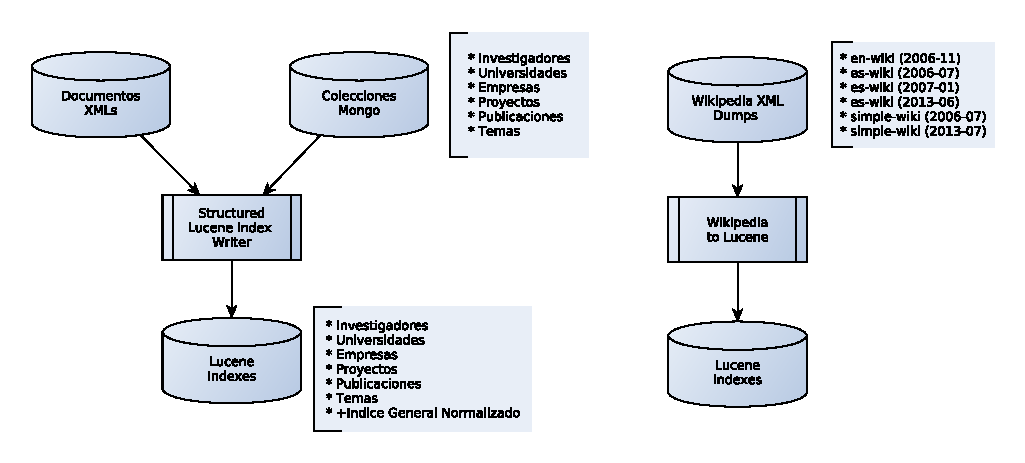
\includegraphics[scale=0.86]{graficos/LuceneWritersJuntos}
  \caption{Creación de Indices}
  \label{fig:LuceneIndexWriterBoth}
\end{figure}

A partir de esta base de datos de mongo y de los archivos xml fueron construidos cinco índices
de búsqueda lucene y un índice de búsqueda más, general, con la
información normalizada de los otros cinco. 
Cada uno de los cinco índices por entidad mantiene la estructura del tipo como campos de los documentos.
Esto quiere decir que el índice invertido para \emph{Investigadores} tiene los mismos campos
del modelo de datos de nosql. Además, se agregó el campo ``all" que resulta de la concatenación de
todos los campos. Este campo resulta útil a la hora de filtrar resultados. 
El índice general posee un documento por cada entidad de las cinco colecciones, 
manteniendo también un puntero a la entidad original y su tipo.
%El proceso de creación de índices se ilustra en la Figura \ref{fig:LuceneIndexWriterEstructurado}%~\nameref{fig:LuceneIndexWriterEstructurado}.

% \begin{figure}[H]
%   \centering
%     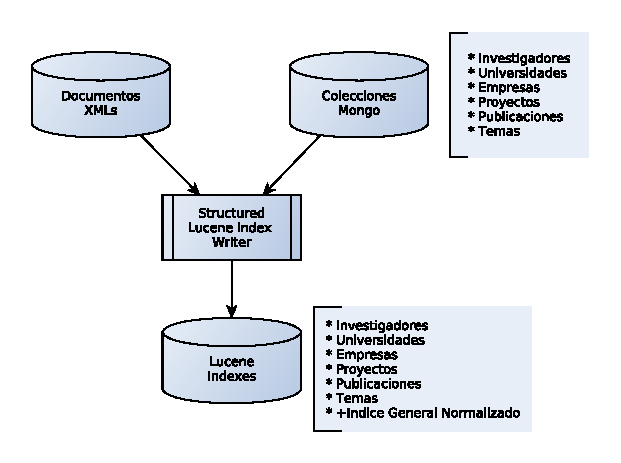
\includegraphics{graficos/LuceneIndexWriterEstructurado}
%   \caption{Lucene Index Writer para datos del proyecto Mitic}
%   \label{fig:LuceneIndexWriterEstructurado}
% \end{figure}

Para la construcción de indices lucene con los dumps de wikipedia usamos la librería gwtwiki (Ver Apéndice~\ref{sec:gwtwiki}).
Los artículos se indexan como documentos con los siguiente campos: \emph{id, title, body y all}. En este proceso se descartan artículos mal formados y 
entradas representado imágenes o discusiones, tal como se sugiere en la guía. 
Por mera curiosidad, tomamos tiempos en la contrucción de estos índices locales sobre versiones de wikipedia.
Estos son algunos tiempos de indexación para distintos dumps sobre una [[detalles de la compu]]:
\begin{center}
\begin{tabular}{| l | l | l | l |}
\hline
Idioma & Tamaño & \# Entradas & Tiempo \\ \hline
es & 50M & \# 16 millones & 2.5min \\ \hline
es & 50M & \# 16 millones & 2.5min \\ \hline
es & 50M & \# 16 millones & 2.5min \\ \hline
es & 50M & \# 16 millones & 2.5min \\ \hline
\end{tabular}
\end{center}

El proceso de creación de índices está ilustrado en la figura \ref{fig:LuceneIndexWriterBoth}



% \begin{figure}[H]
%   \centering
%     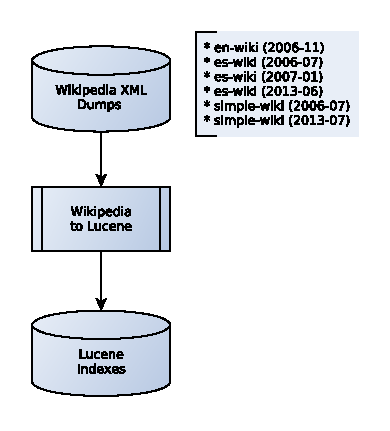
\includegraphics{graficos/LuceneIndexWriterWiki}
%   \caption{Lucene Index Writer para dumps de Wikipedia}
%   \label{fig:LuceneIndexWriterWiki}
% \end{figure}



\subsection{Interfaz de servicios}
\label{subsec:modelos-db}
La creación offline de índices lucene tiene como finalidad optimizar
la base de conocimiento para responder con mayor eficiencia 
a búsquedas de resultados en un momento posterior. 

En esta sección vamos a ver la interfaz que presenta la base de conocimientos indexada 
al resto de los módulos del sistema y qué dependencias existen con los módulos de
análisis lingüístico.

Para la base de conocimiento estructurada, reutilizamos un modelo de datos
escrito en java  del grafo de entidades que obtuvimos de los investigadores del proyecto mitic (Ver \allref{sec:modelos-morphia}).
A estos modelos se les agregó soporte para su representación como documento dentro de un índice.
Por ejemplo, el modelo para la entidad ``Universidad de Buenos Aires", además de
persistirse en la colección de universidades de la base de datos de mongo, también dispone de una representación como documento en 
un índice lucene particular (el índice de universidades) y otra en el índice general.
A nivel colecciones, cada entidad dispone de un representante que maneja el acceso a su colección en la base de datos y también a su índice. A partir de estos representantes por entidad que ofrecen acceso a una base de datos y a un índice creamos la interfaz \emph{KnowlegdeBase}. 
Cada entidad tiene una interfaz de administración de sus dos motores de persistencia. Las responsabilidades de esta interfaz son las de un handler de conocimiento acerca de una cierta clase de entidades. 
Además, esta interfaz permite la reificación de entidades implicitas en el modelo. Estas entidades son: Ciudad, Provincia, Centro de Investigación, etc \footnote{hacer y escribir bien}. Esta reificación significa abstraer las funciones directas contra la base de datos. Mientras el $KnowledgeBase$ de Investigadores habla directo contra la base mongo o contra lucene, el $KnowlegdeBase$ de Ciudades habla contra Investigadores, Universidades y Empresas verificando ciertos campos y recomponiendo la forma de la entidad, de modo abstracto y sin persistencia propia. 

[[Tablita con totales por entidad]]

\bigskip

[[Relaciones solo presentes en mongo]]

\bigskip

Las $KnowledgeBase$ de las cinco entidad y el índice general están, a su vez, controlados un $KnowlegdeManager$, que es la interfaz del módulo que maneja la base de conocimiento. 

El $KnowledgeManager$ ofrece diferentes servicios de verificación de entidades. Para una cadena de tokens cualquiera, este módulo puede decidir, con un cierto grado de confianza, los siguientes problemas:

\begin{itemize}
  \item Si la cadena de tokens es una entidad dentro del modelo de datos. Esto incluye:
    \begin{itemize}
      \item Es una entidad del modelo de datos: una universidad, una empresa, un investigador, un proyecto, una publicacion o una tematica
      \item Es una entidad inferida: una ciudad, una provincia, un centro de investigación, un lugar de trabajo
    \end{itemize}
  \item Si la cadena es una colección del modelo de datos, es decir, si se están nombrando \dblquote{Investigadores} o \dblquote{Universidades} como clase de entidades.
  \item Si la cadena es un atributo o una relación de una clase de entidades.
\end{itemize}

La primer verificación utiliza campos de identidad de las entidades y diferentes tipos de comparadores (Ver apéndice \allref{sec:comparadores} ). Cada entidad fue configurada con diferentes atributos de identidad y a su vez estos atributos están asociados a diferentes comparadores a con un cierto grado de peso y de confianza en el juicio general. 

La segunda y la tercera verificación utiliza estos mismos comparadores jerarquizados, pero compara las cadenas de entrada contra diccionario de sinónimos escrito a mano nombrando las diferentes clases de entidades y los atributos de cada una de ellas. 

\begin{figure}[H]
  \centering
    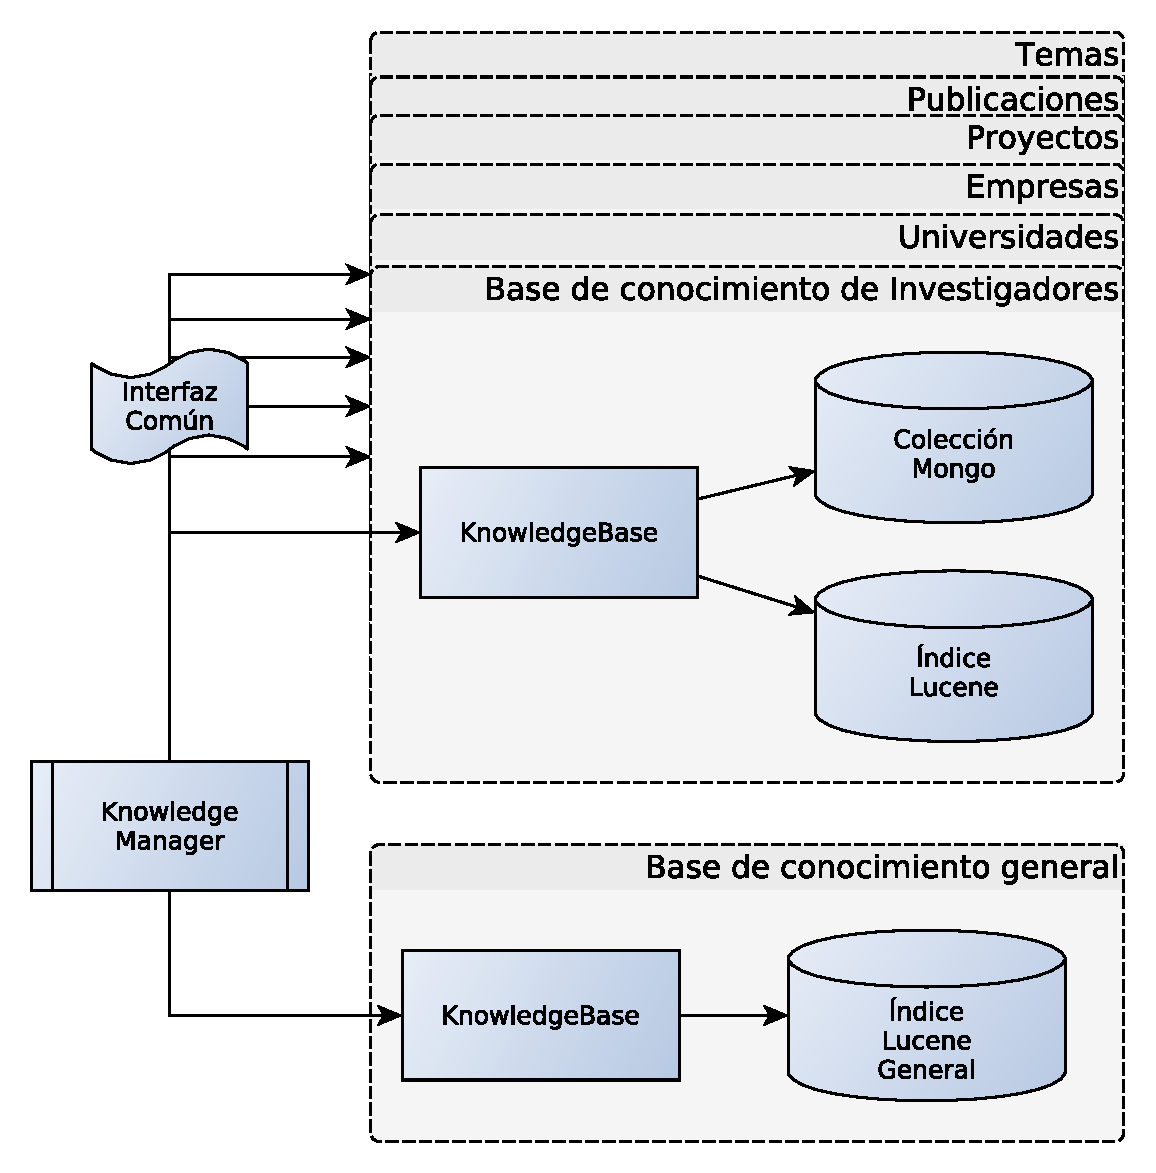
\includegraphics[scale=0.5]{graficos/KnowledgeManager}
  \caption{Base de Conocimiento de grafo de TICs}
  \label{fig:KnowledgeManager}
\end{figure}

\bigskip

La base de conocimiento de los ejercicios de Clef '07 es mucho más sencilla 
porque no existe ningún modelo \emph{a priori} más allá del documento de lucene.
El formato de la entidad ``artículo", como señalamos antes, es: $(id, titulo, cuerpo)$. 
En este caso, el trabajo más fino no está en el modelado inicial del dominio 
sino la capacidad lingüística de extraer pasajes a partir de un artículo y recomponer información
estructurada a partir de estos pasajes. Mientras que para un modelo estructurado la base de conocimiento
debería permitirnos, para un cierto input, identificar univocamente una entidad y darnos pistas sobre un pedido de
información acerca de esa entidad, el objetivo sobre un corpus de documentos en 
traer todos los documentos en los que sea posible que exista un pasaje respondiendo a la pregunta o
evidencia relevante para apoyar una respuesta. Es decir, mientras una respuesta acotada es una virtud para
el manejador de una base de conocimientos estructurada, el manejador de una lista de documentos de texto debería devolver
una lista lo suficientemente grande para contener la respuesta dentro de los pasajes. La razón de esta política es que si
por ser demasiado estrictos a la hora de retornar documentos llegasemos a descartar un pasaje candidato válido esto
redundaría en una baja generar de efectividad, mientras que en pasos subsiguiente será trivial descartar toda información irrelevante
sin tanto costo. Por eso, el acceso a los indices de wikpedia consta simplemente de un generador de queries similar al recién comentado
accediendo y acumulando resultados (rankeados) a partir de un $LuceneIndexReader$ común (Ver \ref{sec:lucene} \nameref{sec:lucene} para más información).


\bigskip

\section{Análisis de la pregunta}
\label{sec:qprocess}
En este paso se realizan diferentes análisis lingüísticos de la pregunta.
El resultado son distintas características asociadas a la pregunta (anotaciones)
y distintas entidades semánticas reconocidas útiles para el proceso de generación de respuestas. 
Las herramientas de procesamiento de lenguaje natural que utilizamos en 
la implementación de este paso del pipeline 
incluyen: detección de lenguaje, extracción y verificación de entidades nombradas (NER), 
de verbos, sustantivos, qwords (qué, quién, cómo) (POS), análisis de n-gramas y categorización por tipo de pregunta (QC).

El proceso de análisis de la pregunta es bastante similar para ambos approachs (estructurado y no estructurado), por lo
que comentaremos ambos en simultaneo, mencionando diferencias cuando corresponda. 
Estructuraremos esta parte de la tesis en las siguientes secciones:

\begin{itemize}
\item Detección de idioma 
\item Detección y verificación de entidades nombradas
\item Análisis gramatical
\item Clasificación del tipo de pregunta
\end{itemize}

Si bien es cierto que el segundo item está basado principalmente en NER-tagging, el tercero en POS-tagging y el cuarto en Question Clasiffication, 
cada uno de estos pasos utiliza estas herramientas de diferentes maneras. Por ejemplo, para la detección y verificación de entidades del analisis estructurado, además del NER-tagger también utilizamos la base de conocimiento y el análisis gramatical y, para el español, la clasificación del tipo de pregunta se hace apoyandose en las qwords identificadas por el POS-tagger.

\subsection{Idioma}

\begin{figure}
  \centering
    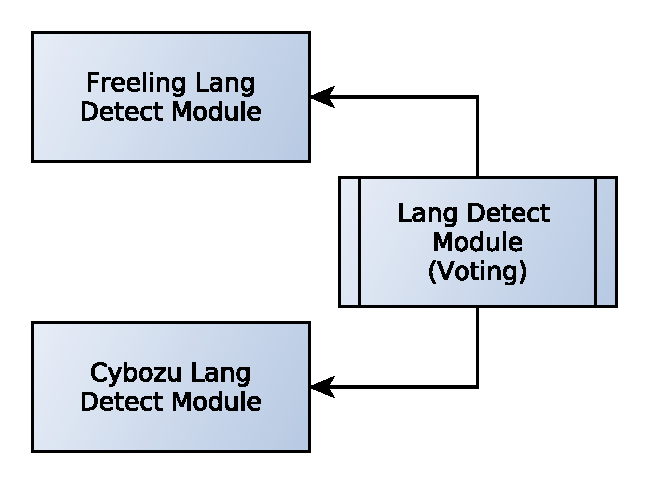
\includegraphics[scale=0.5]{graficos/LangDetect}
  \caption{Módulo de Detección de Idiomas}
  \label{fig:LangDetect}
\end{figure}

El módulo de detección de idiomas de nuestro sistema utiliza dos librerías distintas.
El módulo de detección de idiomas de Freeling y una librería especializada de Cybozu Labs. (Ver apéndices \allref{sec:freeling} y \allref{sec:cybozu} para más información)

Ambos permiten priorizar la detección de ciertos idiomas sobre otros desde su configuración.
De esta manera podemos forzarlos a identificar sólo los idiomas esperados en nuestro dominio. 
Ambos fueron configurados para detectar inglés y español para mejorar la confiabilidad,
pero pueden habilitarse más idiomas de ser necesario y funcionan correctamente. 

El módulo de detección simplemente evalua ambos algoritmos y 
decide el resultado con un cierto grado de confianza. En caso de existir un empate, se 
prioriza la opción de Cybozu labs que en la práctica dió resultados más exactos.

De todos modos, el problema "detección de idioma" no introduce mayores complicaciones y parece un problema bien resulto.
Es decir, la mayoría de las veces ambos módulos responden lo mismo y de modo correcto.
Sin embargo, para ciertos casos bordes molestos (pero lamentablemente frecuentes)
el detector de Cybozu resultó funcionar mejor. Por ejemplo, está el caso de la pregunta formulada en inglés pero acerca de una entidad nombrada en español: 
``Where is located the Universidad de Buenos Aires?". Este problema está particularmente presente en el procesamiento de preguntas -nuestra tarea-, dado que son textos cortos en los que una construcción sustantivada en otro idioma puede desequilibrar erróneamente la balanza. 

A continuación presentamos algunos ejemplos que ilustran el funcionamiento de ambas librerías y el resultado final de nuestro módulo en estos casos:

\begin{center}
\begin{tabular}{| p {8cm} | l | l | l |}
\hline
Texto & Freeling & Cybozu & Resultado \\ \hline
¿Dónde queda la Universidad de Buenos Aires? & es & es & es \\ \hline
Where is located the University of Buenos Aires? & en & en & en \\ \hline
Where is located the Univesidad de Buenos Aires? & en & en & en \\ \hline
Where is located Universidad de Buenos Aires? &  {\color{red}es} & en & en \\ \hline
Quién es Carolina Fernandez? & es & es & es \\ \hline
Who is Carolina Fernandez? &  {\color{red}none} & en & en \\ \hline
Quién es John McCain? & {\color{red}none} & es & es \\ \hline
Who is John McCain? & en & en & en \\ \hline
Dónde vive John McCain y por qué vive allí? & es & es & es \\ \hline
Where does Carolina Fernandez live and why does she lives there? & en & en & en \\ \hline
\end{tabular}
\end{center}

Los ejercicios de Clef '07 no evaluan detección de idiomas. Los archivos de preguntas están separadas por idioma y no se espera que el idioma se infiera a partir de los textos de las preguntas, sino que es un dato dado al sistema de QA.

\subsection{Entidades nombradas}
\label{subsec:impl-ner}

Para la detección de entidades utilizamos la clase simple de detección (NER) y clasificación (NEC) de entidades de Freeling y el NERC de Stanford (ver \allref{sec:freeling} y \allref{sec:stanford-ner}). Las herramientas de Stanford en general superan a las de Freeling -al igual que el detector de idiomas de Cybozu-, pero solo sirven para inglés. La clasificación utilizada por ambos es la más general de las comentadas en \allref{subsec:nerc}: persona, lugar, organización y otros. 

Veamos algunos ejemplos de funcionamiento de los módulos de detección de entidades. 

\begin{center}
\begin{tabular}{| p {8cm} | l | l | l |}
\hline
Texto & Freeling & Stanford & Resultado \\ \hline
¿Dónde queda la Universidad de Buenos Aires? & es & es & es \\ \hline
Where is located the University of Buenos Aires? & en & en & en \\ \hline
Where is located the Univesidad de Buenos Aires? & en & en & en \\ \hline
Where is located Universidad de Buenos Aires? &  {\color{red}es} & en & en \\ \hline
Quién es Carolina Fernandez? & es & es & es \\ \hline
Who is Carolina Fernandez? &  {\color{red}none} & en & en \\ \hline
Quién es John McCain? & {\color{red}none} & es & es \\ \hline
Who is John McCain? & en & en & en \\ \hline
Dónde vive John McCain y por qué vive allí? & es & es & es \\ \hline
Where does Carolina Fernandez live and why does she lives there? & en & en & en \\ \hline
\end{tabular}
\end{center}

\medskip

Mientras la detección de entidades para los ejercicios de Clef se detiene en el reconocimiento de entidades nombradas a nivel lingüísitico, para el sistema estructurado el proceso es un poco más complejo. Esto se debe a que en este caso la detección de entidades es esencial. Si en el proceso de anotado de la pregunta no se logra identificar alguna entidad reconocida por el modelo de datos, entonces se está muy lejos de encontrar una respuesta. Por eso, además de utilizar los modulos NER recién mencionado, agregamos otros algoritmos de detección y, también, verificación de entidades. 

En principio, verificamos la o las entidades nombradas reconocidas contra la base de conocimiento. El $KnowledgeManager$ ofrece diferentes servicios de verificación de entidades. Para una cadena de tokens cualquiera, este módulo puede decidir, con un cierto grado de confianza, si:

\begin{itemize}
  \item La cadena de tokens es una entidad dentro del modelo de datos. Esto incluye:
    \begin{itemize}
      \item Es una entidad del modelo de datos: una universidad, una empresa, un investigador, un proyecto, una publicacion o una tematica
      \item Es una entidad inferida: una ciudad, una provincia, un centro de investigación, un lugar de trabajo
    \end{itemize}
  \item La cadena es una colección del modelo de datos, es decir, si se están nombrando \dblquote{Investigadores} o \dblquote{Universidades} como clase de entidades.
  \item La cadena es un atributo o una relación de una clase. (nombre de investigador)
\end{itemize}

Parte importante del trabajo para este esquema es lograr identificar este tipo de entidades lingüísticas, por lo que además de verificar los resultados del proceso de NER-tagging, también generamos otras cadenas de input. Notar además que los nombres de clase y de atributos de clase no tendrían por que ser reconocidas por el NER-tagger. Por ejemplo, para ``¿Qué investigadores trabajan en Córdoba?", \dblquote{investigadores} está haciendo referencia al nombre de una clase pero no es el tipo de entidades lingüísticas que detecta un NER-tagger. 

Por estas razones, generamos más entidades lingüísticas posibles además de las entidades detectadas por los NER-taggers. Una vez que todas las entidades nombradas fueron verificadas, generamos n-gramas sobre el resto de la pregunta para chequear por más tokens reconocibles. Configuramos la generación de n-gramas de 1 a 3, con ciertos filtros para no verificar construcciones que no representan entidades de manera trivial. Por ejemplo: dejamos sólo los unigramas que cumplan el rol de sustantivos, eliminamos bigramas que sean un sustantivo y una acción, salteamos NERs ya reconocidas, etre otros.


\subsection{Análisis gramatical}

De las diferentes etiquetas que generan los POS-taggers, en nuestro sistema distinguimos los verbos, los sustantivos, las qwords y las palabras triviales. 
Las palabras etiquetadas cumplen distintos roles a lo largo del proceso de generación de respuestas. Como señalamos recién, los n-gramas que se verifican contra la base de datos están filtrados por los roles gramaticales de sus tokens. Por otro lado, a la hora de generar el tipo de pregunta para una pregunta en español, utilizamos, como mecanismo ad-hoc, las qwords. 

\begin{center}
\begin{tabular}{| l | l |}
\hline
Clase & Ejemplos\\ \hline
qword  & qué, quién, cómo, dónde, cuándo\\ \hline
verbo & trabaja, trabajar, trabajando \\ \hline
trivial  & lo, a, de, y \\ \hline
sustantivos  & universidad, impresora, álgebra \\ \hline
\end{tabular}
\end{center}

Los usos más intensivos de estas etiquetas son el filtrado de n-gramas que describimos en la sección anterior para el caso estructurado (\allref{subsec:impl-ner}), un algoritmo ad-hoc de etiquetado de Q-Type para el caso español (es el próximo tema a discutir en \allref{subsec:qtype}) y, para la generación de respuestas, las ponderaciones de pasajes en los scorers de los ejercicios de Clef (\allref{subsec:scorers}), y finalmente, sirven para desempatar por atributos o relaciones preguntadas en algunos casos del modelo estructurado.

\subsection{Clasificación}
\label{subsec:qtype}
Para clasificar la pregunta según su tipo de respuesta esperada utilizamos el Question Classiffier de Stanford, tomando la configuración de Qanus. Este clasificador arroja una clase y una subclase (ver \allref{sec:stanford-qc} para una lista detallada de las posibles clases) y un grado de confianza para esta asignación. A continuación presentamos algunos ejemplos que ilustran estos resultados.

\begin{center}
\begin{tabular}{| l | l | l |}
\hline
Pregunta & Clase y Subclase & Confianza\\ \hline 
What's his name? & HUM:ind & 0.74 \\ \hline 
Where do you come from? & DESC:desc & 0.62 \\ \hline 
What's your phone number? & NUM:code & 0.63 \\ \hline 
How old are you? & NUM:period & 0.78 \\ \hline 
When were you born? & NUM:date & 0.99 \\ \hline 
What does he look like? & DESC:desc & 0.82 \\ \hline 
\end{tabular}
\end{center}

Sin embargo, como ya señalamos oportunamente (ver \allref{subsec:qc}), no existen herramientas de clasificación de preguntas para el idioma español. Esto nos llevó a tomar diferentes medidas para aproximar un tipo de pregunta y no tener distintos casos de código para el inglés y el español. Para las preguntas de Clef formuladas en español, utilizamos su versión en inglés para obtener el tipo.
Así, el tipo de respuesta esperada de \dblquote{¿En qué colegio estudia Harry Potter?} es el mismo que el tipo de respuesta esperada de ``In what school does Harry Potter study?" (ENTY:cremat con 0.22 de confianza). Además, utilizamos reglas escritas a mano sobre QWords. Las qwords son palabras clave de las preguntas que señalan el tipo de respuesta. Por ejemplo: una pregunta que comienza con `Cuándo' tendrá como tipo de respuesta una fecha, un tiempo, etc. En el modelo estructurado, definimos una serie acotada de categorías de tipo de respuesta esperadas y unificamos los resultados del clasificador de Stanford y nuestras reglas sobre qwords para español para unificar el código. Estas categorías son:  Who, Whom, Where, Which,  When,  What y Other. Es decir: Quién, Quiénes, Dónde, Cuál, Cuándo, Qué y otros. Las clases y subclases del clasificador de Stanford se mapearon a estas categorías que coinciden con los resultados de las reglas escritas a mano para el español. 


\subsection{Entidad de Grupo}
\label{subsec:entidad-de-grupo}

El formato de las preguntas para los ejercicios Clef que elegimos es un xml para cada idioma. En particular, nosotros resolvimos los ejercicios en español y inglés que podían responderse en base a wikipedia. Contar del tema de los grupos. Poner algún ejemplo.

\section{Generación de Respuestas}

El proceso de generación de respuestas difiere sustancialmente entre ambos modelos de dominio. Para el sistema basado en datos estructurados, el approach es determinan en casos de código las distintas posibilidades, acotadas, de las cosas que se pueden responder. Nuestro dominio es tal que solo se pueden responder entidades, atributos de entidades o relaciones entre entidades. De ese modo, si no es posible redirigir el flujo de la pregunta hacia alguna respuesta conocida, no hay posibilidad de articular una respuesta significativa. Para el caso de los ejericicios de Clef sobre wikipedia, el enfoque es muy distinto. En primer lugar, no hay un modelo de los datos del dominio, hay textos con pasajes (u oraciones). Si bien es posible una cierta jerarquización de los datos (por ejemplo, utilizando los nombres de los articulos como verificación de la existencia de una entidad), un enfoque estructurado resulta imposible. En este contexto se utiliza la técnica de rankeo semántico de pasajes en base a features (características). Estas dimensiones de valoración de los pasajes son llamados Scorers (ver \allref{subsec:scorers}). Los Scorers, como veremos, pueden ser tan sencillos como preferir minimamente una cierta longitud sobre otra y también pueden incorporar dimensiones de análisis lingüístico (por ejemplo, la presencia de cierta entidad en un cierto rol semántico). El algoritmo de generación de respuestas consiste, en el caso no estructurado, en encontrar features útiles, significativos y en establecer mecanismo inteligentes de priorización de estos features. 

\subsection{Estructurado}

Una vez etiquetados todos los tokens de la pregunta, se procede a marcar como procesadas las ``palabras triviales". Estas son palabras que si no formaron parte de alguna otra construcción, entonces no haberlas procesado no debería considerarse un problema. Ejemplos de ellas son las proposiciones, los pronombres y algunos conectores. Si al etiquetar la pregunta no se logró identificar ninguna entidad del modelo, entonces será dificil avanzar. Como vimos recién, la fase de procesamiento de la pregunta para el caso estructurado excede por mucho la mera anotación lingüística: al finalizar el etiquetado deberíamos disponer de alguna entidad reconocida por el modelo. Por otro lado, durante la fase de etiquetado cada palabra se marca como procesada. Como acabamos de señalar, al finalizar este proceso se marcan también como procesados ciertos tokens triviales. En este punto, el sistema debe tomar una decisión. Si no ha logrado etiquetar una cierta cantidad de tokens (más del 80\%), entonces se considera que no tiene sentido dar por ``comprendida" la pregunta y se procede a un segundo análisis, computacionalmente más costoso y además más inexacto, en el que se intenta encontrar alguna entidad con otros métodos que enunciaremos en breve. En caso de encontrarse una entidad, entonces el flujo del programa retorna al curso de análisis estructurado. Si esto no ocurre, se devuelve la lista de entidades (documentos) que el índice lucene general devuelve para la pregunta original interpretada como una query normal de information retrieval. Este caso, si bien retorna información, es un caso de falla de procesamiento. Esta lista de documentos viene acompañada de un mensaje del tipo: \dblquote{No se logró interpretar su pregunta} y, en un trabajo futuro, podría incorporar un sistema de recomendaciones e idas y vueltas con el usuario (¿Quizo decir...?).

Si, en cambio, el threshold de tokens es alcanzado, entonces se pasa a otro switch. En este caso el código se bifurca de acuerdo a la cantidad de entidades del modelo reconocidas. Por entidades del modelo entenderemos, aquí, entidades internas, objetos, no nombres de clase o de atributos. Distinguimos estos tres casos: `ninguna entidad reconocida', `una entidad reconocida', `más de una entidad reconocida'.


\begin{figure}[H]
  \centering
    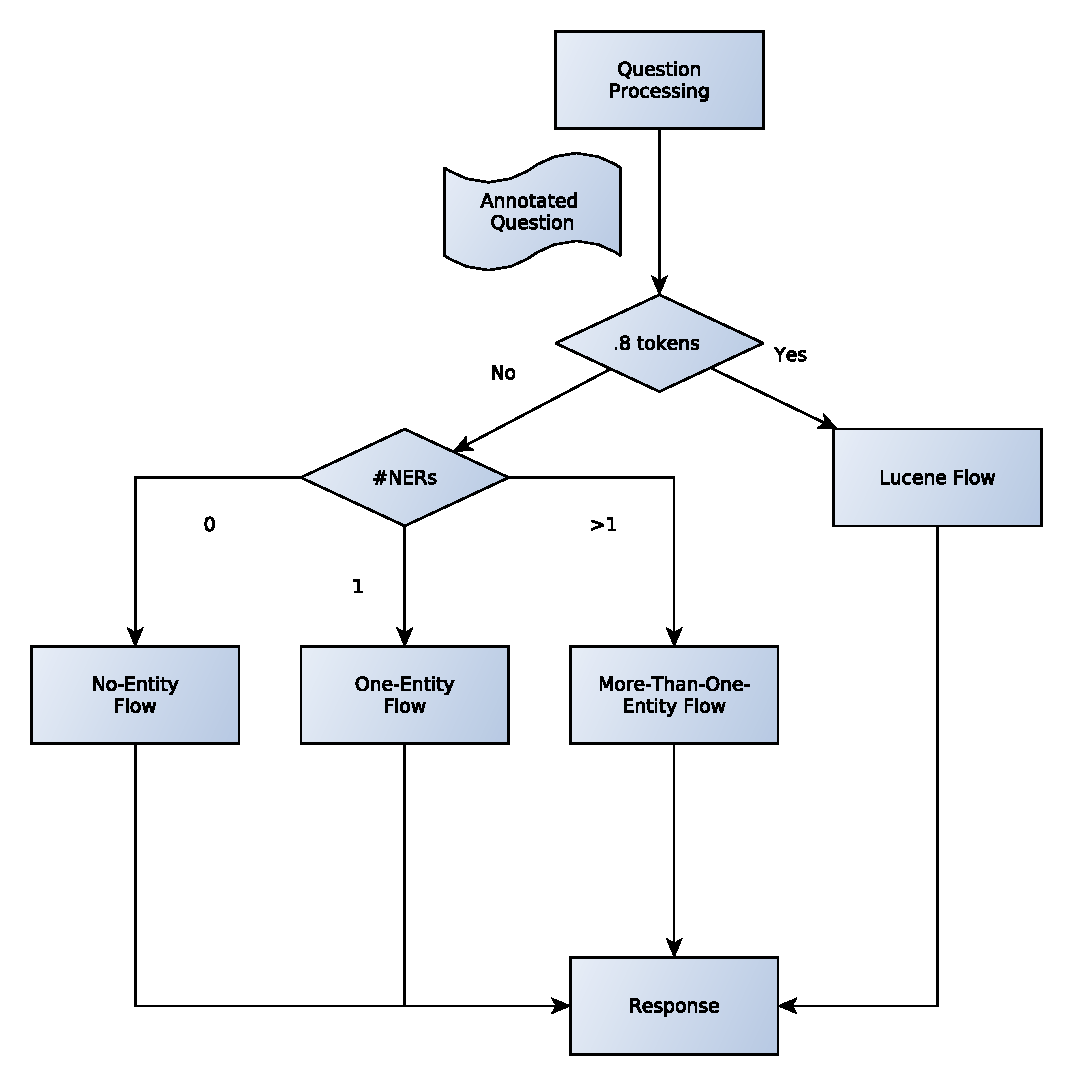
\includegraphics[scale=0.5]{graficos/AnswerRetrievalFlowEstructurado}
  \caption{Flow para la Generación de Respuestas - Estructurado}
  \label{fig:AnswerRetrievalFlowEstructurado}
\end{figure}

\subsubsection*{Ninguna o más de una entidad}
En el caso en el que no se haya identificado ninguna entidad del modelo quedan diferentes posibilidades, que se verifican en orden secuencial en base a nombres de colección, nombres de atributos, tipo de respuesta esperada y verbos. Los casos contemplados son: la pregunta por un campo de una colección (por ejemplo: direcciones de empresas en buenos aires) o por listas de entidades de una colección (investigadores de capital federal). Los diferentes casos son reglas de código escritas a mano. En todos los casos, si no se dan las condiciones para seguir especificando la dirección de la respuesta, se genera un respuesta ad-hoc con datos rankeados según el índice invertido, especificando de modo estructurado el camino recorrido hasta el momento. Por ejemplo, si se identifica que se pregunta por `investigadores' pero no es posible decidir ninguna especificación más (de capital federal, que hayan publicado en 2008, etc) entonces se retorna una lista de investigadores rankeada según el índice invertido `investigadores' con el resto de los datos de la pregunta. 

Por otro lado, si hay más de una entidad reconocida entonces hay sólo algunos casos posibles de relaciones entre ellas que pueden ser respuestas, que también se reflejan como caso de código. Finalmente, si no es posible identificar ninguno de estos caso, se toma un camino similar al mecanismo ad-hoc basado en information retrieval.


\subsubsection*{Una entidad}
El mejor caso es aquél en el que se reconocío una entidad y otros datos lingüisticos que permitan especificar qué se está preguntando. Al especificar acerca de qué/quién resulta mucho más sencillo canalizar qué se está preguntando. Los modelos que representan objetos (ver \allref{subsec:modelos-db}) son subclases de $NodoBase$, el cual representa una entidad en abstracto. Una entidad sabe responder preguntas acerca de ella. Para esto, utiliza las anotaciones de verbos, atributos nombrados y qwords para identificar qué se está preguntando. La pregunta puede responderse con un atributo o con una relación. Los distintos atributos de las distintas entidades se corresponden con verbos y con tipos de respuesta esperada. 

[[Detalle de casos y combinaciones de verbos + tipo de respuesta esperada + atributo]]
[[Ejemplos]]

\subsection{No Estructurado}

El proceso de generación de respuestas para los ejercicios de la Clef es muy distinto del anterior y puede dividirse en tres pasos principales: obtención de documentos y pasajes, ranking de pasajes y generación de respuesta. En el primer paso se accede a los índices invertido (al corpus) buscando documentos relevantes. Este paso pertenece netamente al área information retrieval. Como mencionamos al comentar Watson (en particular, ver \allref{subsec:deep-qa}), es fundamental que el resultado de este paso sea lo suficientemente amplio como para contener la respuesta pero lo suficientemente acotado como para no sobrecargar el proceso posterior de análisis lingüístico sobre los pasajes. Los documentos rankeados se dividen en pasajes. En el segundo paso, tanto los documentos como los pasajes son contrastados con distintas métricas contra los datos de la pregunta generando distintos valores para estos features. Finalmente, con esta información se procede al tercer paso, que consiste en realizar diferentes filtrados sobre los pasajes en función del tipo de respuesta esperado y en distintas formas de recopilar evidencia a favor de un pasaje o una entidad (depende el caso) para finalmente seleccionar una respuesta (o decidir que no se encontró ninguna).

\begin{figure}[H]
  \centering
    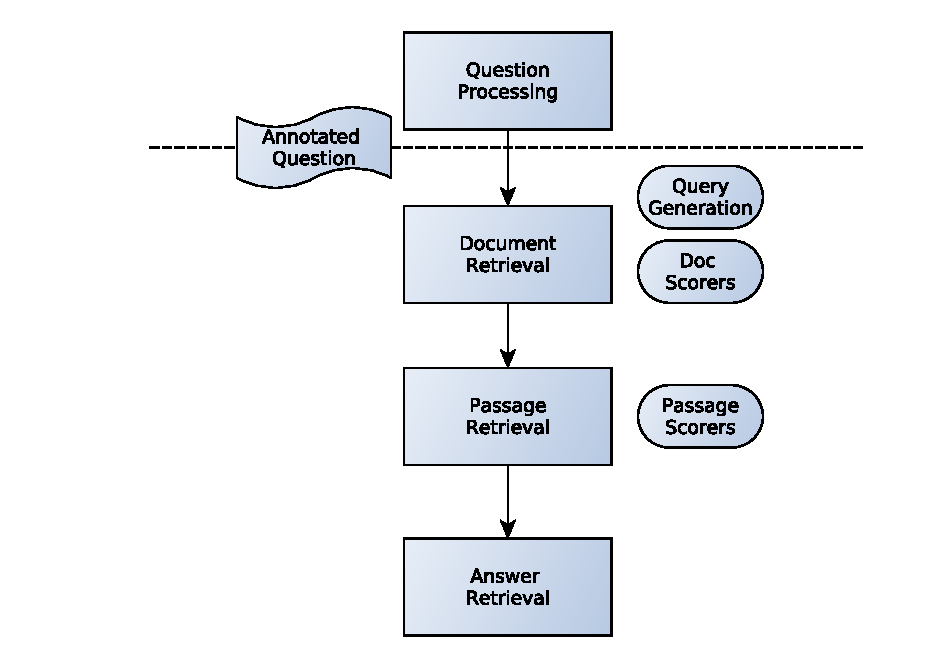
\includegraphics[scale=0.75]{graficos/AnswerRetrievalFlowWiki}
  \caption{Flow para la Generación de Respuestas - No Estructurado}
  \label{fig:AnswerRetrievalFlowWiki}
\end{figure}

\subsubsection{Documentos}
\label{subsec:docs}
En este punto, para una pregunta dada se dispone de la entidad del grupo de preguntas y de las distintas anotaciones hechas a la pregunta en el paso anterior (\allref{sec:qprocess}). Por su parte, los documentos en los índices invertidos poseen los campos $Id$, $Title$, y $Text$. El mecanismo de generación de queries tiene como objetivo priorizar en el ranking los documentos relacionados con el tema asociado al grupo de preguntas. Este paso es un problema de information retrieval puro: esto es, dado un pedido de información, retornar \textit{documentos relevantes}. El análisis semántico tiene peso en el paso posterior, a la hora de rankear pasajes. Por ejemplo, para el primer grupo de preguntas acerca de Harry Potter, solo se espera de este una lista de de documentos relacionados con ese mundo, en primer lugar. Por otro lado, es necesario que los principios de generación de queries no sean demasiado estrictos. Si en este punto quedan afuera muchas ocurrencias de una respuesta, entonces todo el resto del programa se ve afectado de manera irreparable. Es preferible generar documentos de más y luego filtrarlos mediante análisis lingüístico que ser demasiado estrictos y perder respuestas. 
Para lograr esto, ponderamos los documentos en los que las entidades nombradas reconocidas lingüísticamente aparecen en el título, si se dispone de más de una entidad buscamos documentos que mencionen ambos, luego priorizamos los documentos que poseen estas entidades dentro del cuerpo y también consideramos la presencia de verbos en diferentes conjugaciones y de sustantivos que ocurren en la pregunta. Finalmente, agregamos una lista de documentos enviando la pregunta misma como una query.  

Dado que finalmente se realizan queries simples (masivas), cabe preguntarse cual es la razón de la generación de queries y la ponderación de documentos. Esta razón es que en el proceso de ranking de pasajes y evaluación de respuesta se utilizan features basados en el score dado por lucene a los diferentes documentos. Si una mejor posición del documento contenedor del pasaje no implica que el pasaje sea correcto, si en cambio es un indicador de que dicho pasaje se encontró más cerca o más lejos del nucleo temático en el que se esperaba encontrarlo. 

Una vez generada la lista de documentos rankeados según lucene, se procede a analizar algunos features en base a distintos scorers propios. A su vez, estos distintos valores se combinan en una evaluación general del documento, que será utilizada luego a la hora de generar una respuesta. Estas dimensiones buscan en el título y en el artículo diferente medidas sobre las entidades nombradas y sobre la pregunta completa. En concreto, se miden distancias a la entidad nombrada que identifica al grupo de preguntas (ver \allref{subsec:entidad-de-grupo}), las entidades nombradad en la pregunta misma, a la pregunta completa y la respuesta esperada data. Las medidas contra la respuesta esperada -dada por Clef- no pueden usarse para generar la respuesta, pero sí para evaluar la performance del sistema. En el siguiente cuadro se muestran las dimensiones que se consideran sobre los documentos. 

\begin{center}
\begin{tabular}{| l | l | l |}
\hline
Entidad & Campo & Comparador \\ \hline
\multirow{6}{*}{Entidad de Grupo} & \multirow{3}{*}{Título} & Span \\ 
& & Covr \\
& & Freq \\ \cline{2-3}
& \multirow{3}{*}{Texto} & Span \\ 
& & Covr \\
& & Freq \\ \hline
\multirow{6}{*}{Entidades de Pregunta} & \multirow{3}{*}{Título} & Span \\ 
& & Covr \\
& & Freq \\ \cline{2-3}
& \multirow{3}{*}{Texto} & Span \\ 
& & Covr \\
& & Freq \\ \hline
\multirow{6}{*}{Todas las entidades} & \multirow{3}{*}{Título} & Span \\ 
& & Covr \\
& & Freq \\ \cline{2-3}
& \multirow{3}{*}{Texto} & Span \\ 
& & Covr \\
& & Freq \\ \hline
\multirow{6}{*}{Pregunta} & \multirow{3}{*}{Título} & Span \\ 
& & Covr \\
& & Freq \\ \cline{2-3}
& \multirow{3}{*}{Texto} & Span \\ 
& & Covr \\
& & Freq \\ \hline
\multirow{6}{*}{Respuesta} & \multirow{3}{*}{Título} & Span \\ 
& & Covr \\
& & Freq \\ \cline{2-3}
& \multirow{3}{*}{Texto} & Span \\ 
& & Covr \\
& & Freq \\ \hline
Score según índice & -- & -- \\ \hline
\end{tabular}
\end{center}

Los comparadores señalados ($Freq$, $Covr$, y $Span$) se utilizan en distintos lugares de esta tesis y su funcionamiento es explicado en el apéndice \allref{sec:comparadores}. Notar que `Entidades de la pregunta' refiere tanto a aquellas reconocidas por el NER-tagger como a construcciones sustantivadas y que `Pregunta' no es la pregunta bruta sino la priorización de verbos conjugados, sustantivos, adjetivos y entidades. 

El score general del documento es un cálculo ponderado de estas diferentes dimensiones. 

Lucene permite especificar cuántos documentos queremos recuperar. Para evaluar la performance de este paso, utilizamos medida distintos scores en base a la respuesta dada por dada por la conferencia para el ejercicio. Es importante notar que dado que no utilizamos las imagenes de wikipedia de la primera sugerencia, es esperable que las respuesta no estén `tal cual'. 
Evaluamos distintos mecanismos de generación de documentos, con distinta cantidad total, bajo distintas métricas. Para generar documentos, probamos la query trivial $ALL: pregunta$ (1), una un poco mejorada $ALL: entidad_de_grupo pregunta$ (2), secuencias concatenadas de queries tal como las describimos más arriba (3) y varios pedidos separados aplanados en un paso posterior (4). Para los cuatro métodos eliminamos los signos de puntuación. Para medir los resultados, utilizamos los comparadores de presencia exacta y diferentes grados de cobertura de términos (.8, .9 y 1). A su vez, evaluamos distintas imagenes de wikipedia para el español. Es total de preguntas del ejercicio, recordamos, es 200. Los resultados son los siguientes.

\begin{center}
\begin{tabular}{|l|l|l|l|l|l|l|}
\hline
Método & \# Docs & Wikipedia & Exacto & Covr 1 & Covr .9 & Covr . 8 \\ \hline

\multirow{6}{*}{1 - Trivial} & 
\multirow{3}{*}{100} & es - 2006 & 132 & 151 & 152 & 159 \\ 
 &  & es - 2007 & 144 & 159 & 160 & 164 \\
 &  & en - 2006 & x & x & x & x \\ \cline{2-7}
 & \multirow{3}{*}{1000} & es - 2006 & 144 & 167 & 167 & 173 \\  
 &  & es - 2007 & 159 & 177 & 177 & 180 \\
 &  & en - 2006 & x & x & x & x \\ \hline

\multirow{6}{*}{2 - Trivial'} & 
\multirow{3}{*}{100} & es - 2006 & 138 & 156 & 157 & 164 \\ 
 &  & es - 2007 & 151 & 167 & 168 & 171 \\
 &  & en - 2006 & x & x & x & x \\ \cline{2-7}
 & \multirow{3}{*}{1000} & es - 2006 & 147 & 168 & 168 & 174 \\ 
 &  & es - 2007 & 163 & 178 & 178 & 181 \\
 &  & en - 2006 & x & x & x & x \\ \hline
hola & ey &wiki& 137 & 156 & 157 & 160  \\ \hline
\multirow{6}{*}{3 - Inteligente} & 
\multirow{3}{*}{100} & es - 2006 & 127 & 144 & 144 & 150 \\ 
 &  & es - 2007 & 141 & 150 & 151 & 156 \\
 &  & en - 2006 & x & x & x & x \\ \cline{2-7}

 & \multirow{3}{*}{1000} & es - 2006 & 143 & 163 & 163 & 170 \\   
 &  & es - 2007 & 158 & 175 & 175 & 179 \\
 &  & en - 2006 & x & x & x & x \\ \hline

\multirow{6}{*}{4 - Inteligente'} & 
\multirow{3}{*}{100} & es - 2006 & 142 & 160 & 161 & 168 \\ 
 &  & es - 2007 & 157 & 170 & 171 & 174  \\
 &  & en - 2006 & x & x & x & x \\ \cline{2-7}


 & \multirow{3}{*}{1000} & es - 2006 & 147 & 168 & 168 & 174 \\ 
 &  & es - 2007 & x & 158 & x & x \\
 &  & en - 2006 & x & x & x & x \\ \hline
 
\end{tabular}
\end{center}

Conclusión de esto.

\subsubsection{Pasajes}
Este paso es análogo al anterior, pero con mayor detalle y granularidad. Cada documento generado en el paso anterior, con sus diferentes puntajes para 
las dimensiones señaladas, se parten en pasajes u oraciones. Nuevamente, sobre estas oraciones realizamos diferentes mediciones y las combinamos generando
un score final. En esta sección discutiremos las mediciones consideradas y los diferentes métodos de combinación de las mismas. Estos métodos de combinación generan distintos rankings de pasajes. Para evaluar estos rankings, nuevamente, utilizaremos la información disponible sobre las respuestas esperadas, buscando que la respuesta esperada se encuentre entre los $n$ pasajes mejor rankeados.
En primer lugar, las distintos scorers implementados son los siguientes:

\begin{center}
\begin{tabular}{| l | l | l |}
\hline
Comparador & Qué & Dónde \\ \hline
\multicolumn{3}{|c|}{Estadísticos} \\ \hline
Freq & Pregunta & Pasaje \\ \hline
Span & Pregunta & Pasaje \\ \hline
Covr & Pregunta & Pasaje \\ \hline
\#Tokens & -- & Pasaje \\ \hline
\multicolumn{3}{|c|}{Basados en NLP} \\ \hline
Presencia & Entidad de Grupo & Pasaje \\ \hline
Presencia & Entidades de pregunta & Pasaje \\ \hline
Presencia & Verbos de pregunta & Pasaje \\ \hline
Presencia & Sustantivos de pregunta & Pasaje \\ \hline
\multicolumn{3}{|c|}{Para evaluación} \\ \hline
Freq & Respuesta & Pasaje \\ \hline
Span & Respuesta & Pasaje \\ \hline
Covr & Respuesta & Pasaje \\ \hline
\end{tabular}
\end{center}

A estos Scorers se le suman los scores del documento asociado al pasaje (ver \allref{subsec:docs}). 
Sobre estas dimensiones disponibles, intentamos las siguientes combinaciones de priorización:

\begin{center}
\begin{tabular}{|l|l|l|}
\hline
\#& Nombre & Fórmula \\ \hline
1& Simple & $2+2=4$ \\ \hline
2& Respuesta & $2+2=4$ \\ \hline
3& Compleja & $2+2=4$ \\ \hline
\end{tabular}
\end{center}

Y consideramos la ocurrencia de respuestas, de la misma manera que en el apartado anterior (Match Exacto y tres medidas de covertura de tokens: 1, .9 y .8), 
sobre los primeros $n$ pasajes, con $n$ = 1, 5, 10, 20, 50 y 100.

\begin{center}
\begin{tabular}{|l|l|l|l|l|l|}
\hline
Fórmula & \#Docs & Exacto & Covr 1 & Covr .9 & Covr . 8 \\ \hline
\multirow{6}{*}{1} & 1 & x & x & x & x \\  \cline{2-6}
 & 5 & x & x & x & x \\ \cline{2-6}
 & 10 & x & x & x & x \\ \cline{2-6}
 & 20 & x & x & x & x \\ \cline{2-6}
 & 50 & x & x & x & x \\ \cline{2-6}
 & 100 & x & x & x & x \\ \hline
\end{tabular}
\end{center}


\subsubsection{Respuestas}





\begin{figure}
  \centering
    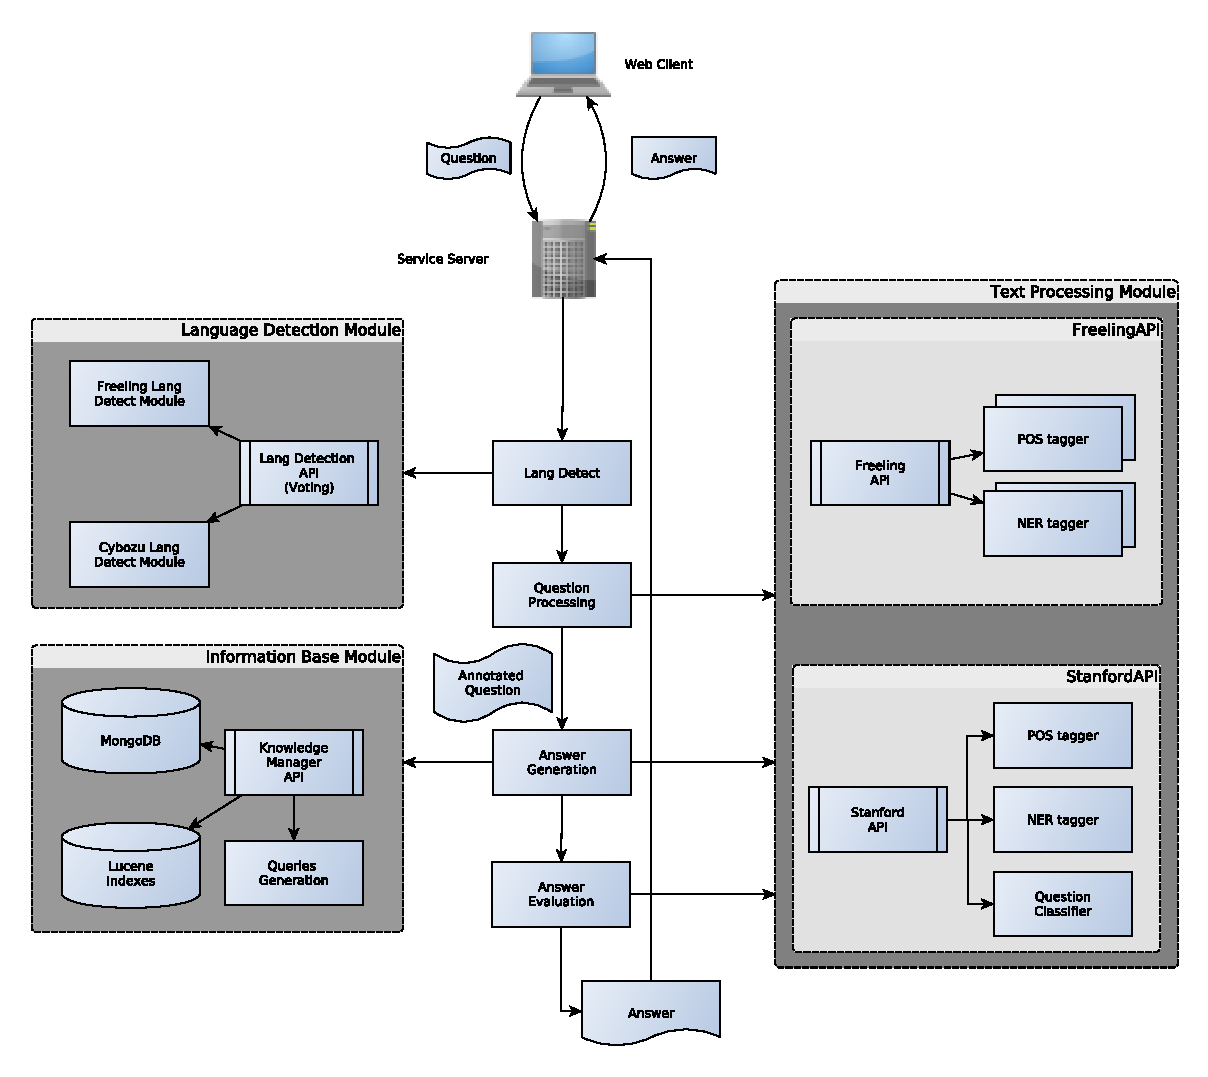
\includegraphics[scale=0.86]{graficos/Architecture}
  \caption{Arquitectura}
  \label{fig:Architecture}
\end{figure}

Como dice en \cite{greenwade93} y también en \cite{RE1}
%\end{document}

%% ...

% \appendix
%\nocite{*}

\begin{appendices}
  \appendix
\chapter{Herramientas}

\section{Stanford Question Classifier}
The question classifier (QuestionClassifier) is implemented with the 
STANFORD CLASSIFIER (Manning and Klein 2003), using the question taxonomy 
explained in (Li and Roth 2002) and is responsible for finding out the expected 
answer type of a given question

Li, Xin, and Dan Roth. "Learning Question Classifiers." International Conference 
on Computational Linguistics (COLING).2002.
Manning, Christopher, and Dan Klein. "Optimization, Maxent Models, and 
Conditional Estimation without Magic." Tutorial at HLT-NAACL and ACL. 2003.

This software is a Java implementation of a maximum entropy classifier.
Maximum entropy models are otherwise known as conditional loglinear
models, and are essentially equivalent to multiclass logistic
regression models (though parameterized slightly differently, in a way
that is advantageous with sparse explanatory feature vectors). 

\section{Stanford POS Tagger}

Part of Speech Tagging Stanford POS Tagger (Toutanova and Manning 
2000)

Toutanova, Kristina, and Christopher Manning. "Enriching the Knowledge 
Sources Used in a Maximum Entropy Part-of-Speech Tagger." Proceedings of 
the Joint SIGDAT Conference on Empirical Methods in Natural Language 
Processing and Very Large Corpora. 2000. 63-70.


\section{Stanford NER Tagger}

Named Entity Recognition Stanford Named Entity Recognizer (Finkel, 
Grenager and Manning 2005)

Finkel, Jenny Rose, Trond Grenager, and Christopher Manning. "Incorporating 
Non-local Information into Information Extraction Systems by Gibbs Sampling." 
roceedings of the 43nd Annual Meeting of the Association for Computational 
Linguistics. 2005.


\section{Freeling}

Freeling es una librer\'ia de c\'odigo abierto que provee distintas herramientas de 
procesamiento de lenguaje natural, desarrollada y mantenida por el Centre de Tecnologies 
i Aplicacions del Llenguatge i la Parla (TALP) de la Universidad Polit\'ecnica de Catalu\~na (UPC). 
Freeling est\'a dise\~nado para ser usada como una librer\'ia externa y ofrece un API en distintos lenguajes
de programaci\'on. Su principal virtud es ser multilingüe, esto es, los diferentes analizadores que provee funcionan 
para un conjunto bastante amplio de idiomas. La \'ultima versi\'on a la fecha (3.1) soporta los siguientes idiomas:

\begin{itemize}
\item Asturian (as)
\item Catalan (ca) 
\item English (en)
\item French (fr) 
\item Galician (gl)
\item Italian (it)
\item Portuguese (pt)
\item Russian (ru)
\item Slovene (sl)
\item Spanish (es)
\item Welsh (cy)
\end{itemize}

Cabe destacar que no todos los m\'odulos soportan todos los idiomas. Sin embargo, dado que el proyecto est\'a radicado en Espa\~na,
los idiomas necesarios para los fines de nuestro trabajo (espa\~nol e ingl\'es), soportan todos los m\'odulos disponibles
en la librer\'ia.
Freeling 3.1 ofrece los siguientes analizadores lingüisticos:

\begin{itemize}
\item Detecci\'on de idioma
\item Tokenizer
\item Sentence splitting,
\item An\'alisis morfol\'ogico
\item NER y NEC (Detecci\'on y Clasificaci\'on de Entidades Nombradas)
\item Reconocimiento de fechas, n\'umeros, magnitudes f\'isicas, monedas
\item Codificaci\'on fon\'etica
\item POS tagging, 
\item Shallow parsing
\item Dependency parsing
\item Wordnet-based sense annotation
\item Word Sense Disambiguation
\item Coreference resolution
\end{itemize}



\section{Lang Detect de Cybozu Labs}

Para la detecci\'on de idiomas utilizamos tanto el m\'odulo que brinda Freeling como una librer\'ia de Cybozu Labs - una reconocida compañ\'ia japonesa,
implementado en Java y liberado bajo Apache License 2.0. En la pr\'actica, este paquete dio excelentes resultados. Soporta 53 idiomas con \%99 de precisi\'on
para todos ellos (seg\'un sus tests). El detector se basa en perfiles de idiomas generados a partir de las distintas wikipedias y detecta el idioma de los texots
usando un filtro bayesiano ingenuo (\textit{naive bayesian}).

\section{MyMemory}
MyMemory es la Memoria de Traducción más grande del mundo: 300 millones de segmentos a finales de 2009

Como las MT tradicionales, MyMemory almacena segmentos con sus traducciones, ofreciendo a los traductores correspondencias y concordancias. El proyecto se diferencia de las tecnologías tradicionales por sus ambiciosas dimensiones y por su arquitectura centralizada y basada en la colaboración colectiva. Todos pueden consultar MyMemory o hacer aportaciones a través de Internet; la calidad de las aportaciones será cuidadosamente ponderada.
MyMemory gives you quick access to a large number of translations originating from professional translators, LSPs, customers and multilingual web content. It uses a powerful matching algorithm to provide the best translations available for your source text. MyMemory currently contains 644.377.834 professionally translated segments.

Las memorias de traducción son almacenes compuestos de textos originales en una lengua alineados con su traducción en otras. Esta definición de memorias de traducción coincide literalmente con una de las definiciones más aceptadas de corpus lingüístico de tipo paralelo (Baker, 1995). Por esto se puede decir que las memorias de traducción son corpus paralelos.


\section{Reverb}

ReVerb is a program that automatically identifies and extracts binary relationships from English sentences. ReVerb is designed for Web-scale information extraction, where the target relations cannot be specified in advance and speed is important.

ReVerb takes raw text as input, and outputs (argument1, relation phrase, argument2) triples. For example, given the sentence "Bananas are an excellent source of potassium," ReVerb will extract the triple (bananas, be source of, potassium).

\section{Apache Lucene}
\label{sec:lucene}
Lucene es una librer\'ia de information retrieval, de c\'odigo abierto, escrita en Java y distribuida 
bajo la licencia Apache Software License por la Apache Software Foundation. No est\'a pensada para
usuarios finales sino para ser integrada dentro de proyectos inform\'aticos, resolviendo
la parte de bajo nivel y brindando servicios a trav\'es de un API en diferentes lenguajes de programaci\'on.
Su core es un \'indice invertido como el que describimos anteriormente. La implementaci\'on de un sistema
que utiliza Lucene consta de dos pasos separados:
\begin{itemize}
\item La \textbf{creaci\'on} del \'indice, es por lo general un proceso offline en el cual 
se incorporan distintas fuentes de informaci\'on al \'indice 
\item La \textbf{b\'usqueda} de documentos en el \'indice creado en el paso anterior, a partir de una query 
ingresada por el usuario final. Este proceso se incorpora dentro del flujo `online' del sistema.
El resultado de esta b\'usqueda es una lista de documentos rankeados con un cierto puntaje. 
\end{itemize}

Es importante señalar que si bien el proceso de creaci\'on del \'indice suele estar desacoplado del resto 
del sistema, las fuentes de informaci\'on no tiene por que ser `offline' en el sentido de ser documentos
en un disco local. De hecho, Nutch, otro proyecto de c\'odigo abierto de la Apache Software Foundation es 
un motor de b\'usqueda web basado en Lucene que incorpora un crawler para indexar sitios web. Lucene soporta 
cualquier fuente de informaci\'on que pueda convertirse en texto mediante algoritmia.
\newline
Los conceptos fundamentales de Lucene son: \'indice, documento, campo, t\'ermino y query.
\begin{itemize}
\item Un \'indice contiene un conjunto de documentos
\item Un documento es un conjunto de campos
\item Un campo es el nombre de una secuencia de t\'erminos
\item Un t\'ermino es un token (una palabra)
\item Una query es una lista de t\'erminos conectados con distintos operados l\'ogicos
\end{itemize}

\bigskip
[[Dar ejemplos de una query]]
\bigskip

\section{gwtwiki -Java Wikipedia API}\label{sec:gwtwiki}

Java Wikipedia API (Bliki engine)
http://code.google.com/p/gwtwiki/
Esta librer\'ia tiene m\'etodos \'utiles para trabajar con dumps de wikipedia. La usamos para testear los m\'etodos no estructurados de la tesis.


\section{Modelos de Morphia}\label{sec:modelos-morphia}

Java Wikipedia API (Bliki engine)
http://code.google.com/p/gwtwiki/
Esta librer\'ia tiene m\'etodos \'utiles para trabajar con dumps de wikipedia. La usamos para testear los m\'etodos no estructurados de la tesis.

  \section{Conclusión}
\section{Trabajo futuro}

\end{appendices}

%%%% BIBLIOGRAFIA
\backmatter
\bibliographystyle{apalike}
\cleardoublepage
\phantomsection
\addcontentsline{toc}{chapter}{Bibliografía}
\bibliography{tesis}


\end{document}
